\documentclass[12pt]{article}
\usepackage{graphicx,amsthm,amsmath,amssymb,algorithm,algorithmic,geometry,setspace,fancyhdr,varwidth,subfig,pdfpages,float}
\usepackage[english]{babel}
\usepackage[colorlinks=true,linkcolor=blue]{hyperref}
\usepackage[superscript,biblabel]{cite}
\usepackage[export]{adjustbox}
\geometry{letterpaper,
	total={170mm,257mm},
	left=20mm,
	top=30mm, bottom=20mm}  % or letter or a5paper or ... etc
% \geometry{landscape} % rotated page geometry

\title{Ph 20: Assignment \#1}
\author{Maya Fuller}
\date{Due: April 9, 2018} % delete this line to display the current date

% See the ``Article customise'' template for come common customisation

\begin{document}
	
	\pagenumbering{gobble}
	
	\maketitle

	\noindent\textbf{\large Problem 3}\\
	\indent\textbf{\large a)}
		\begin{figure}[ht]
			\centering
			\subfloat[$\frac{f_X}{f_Y} = \frac{e}{0.3}$]{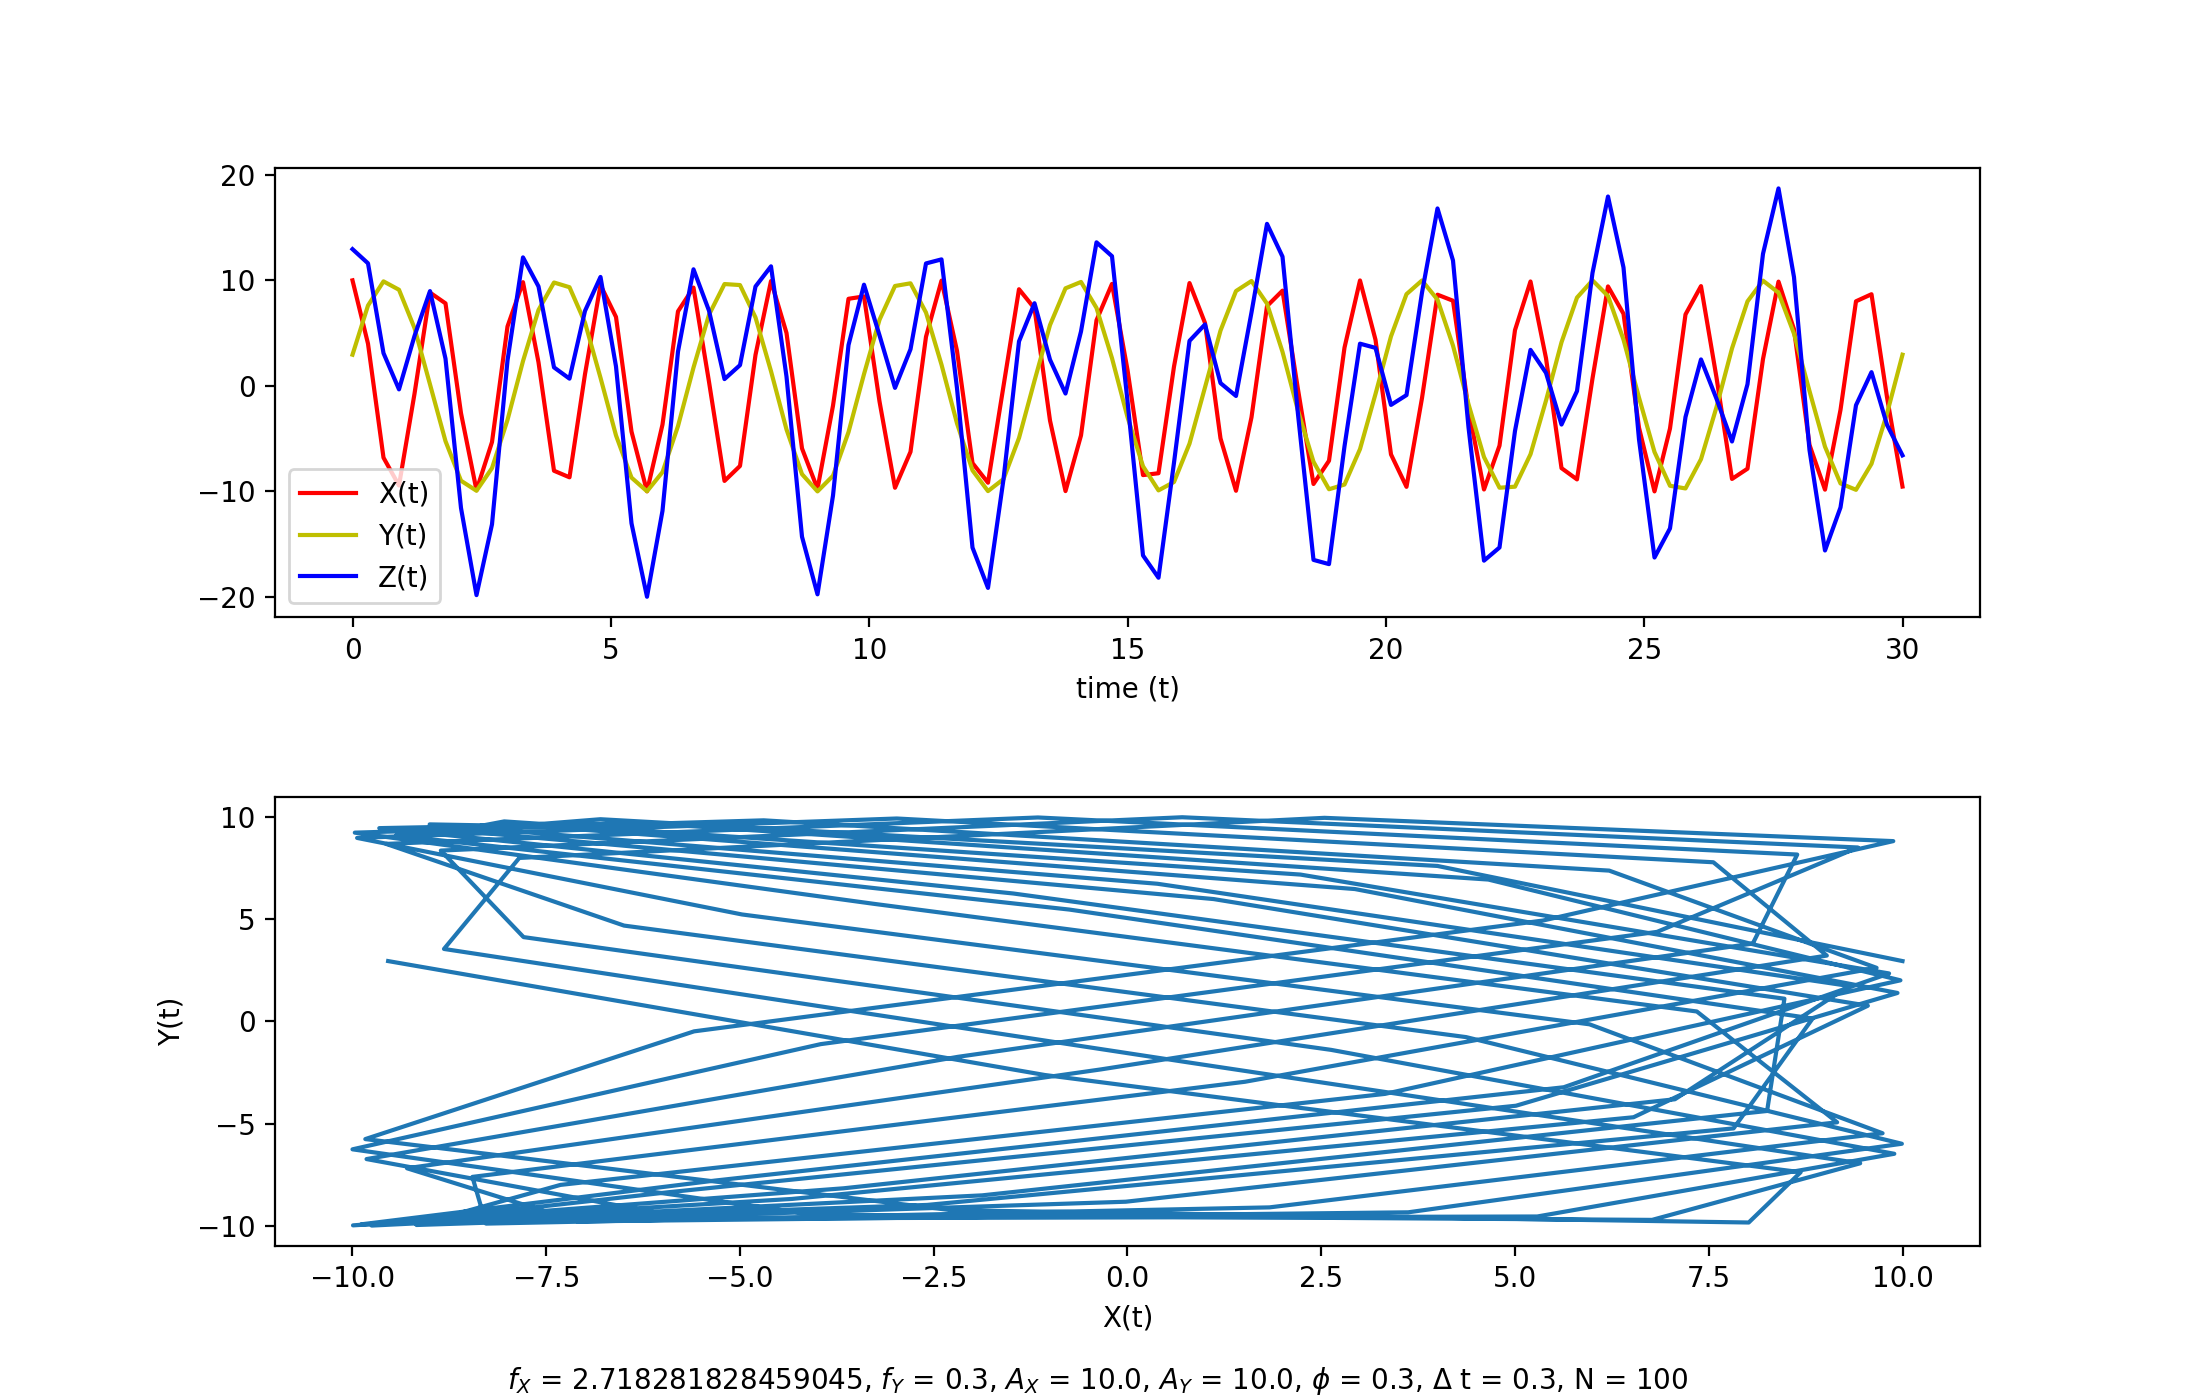
\includegraphics[width=0.48\textwidth]{e3a.png}}
			\subfloat[$\frac{f_X}{f_Y} = \frac{\pi}{0.3}$]{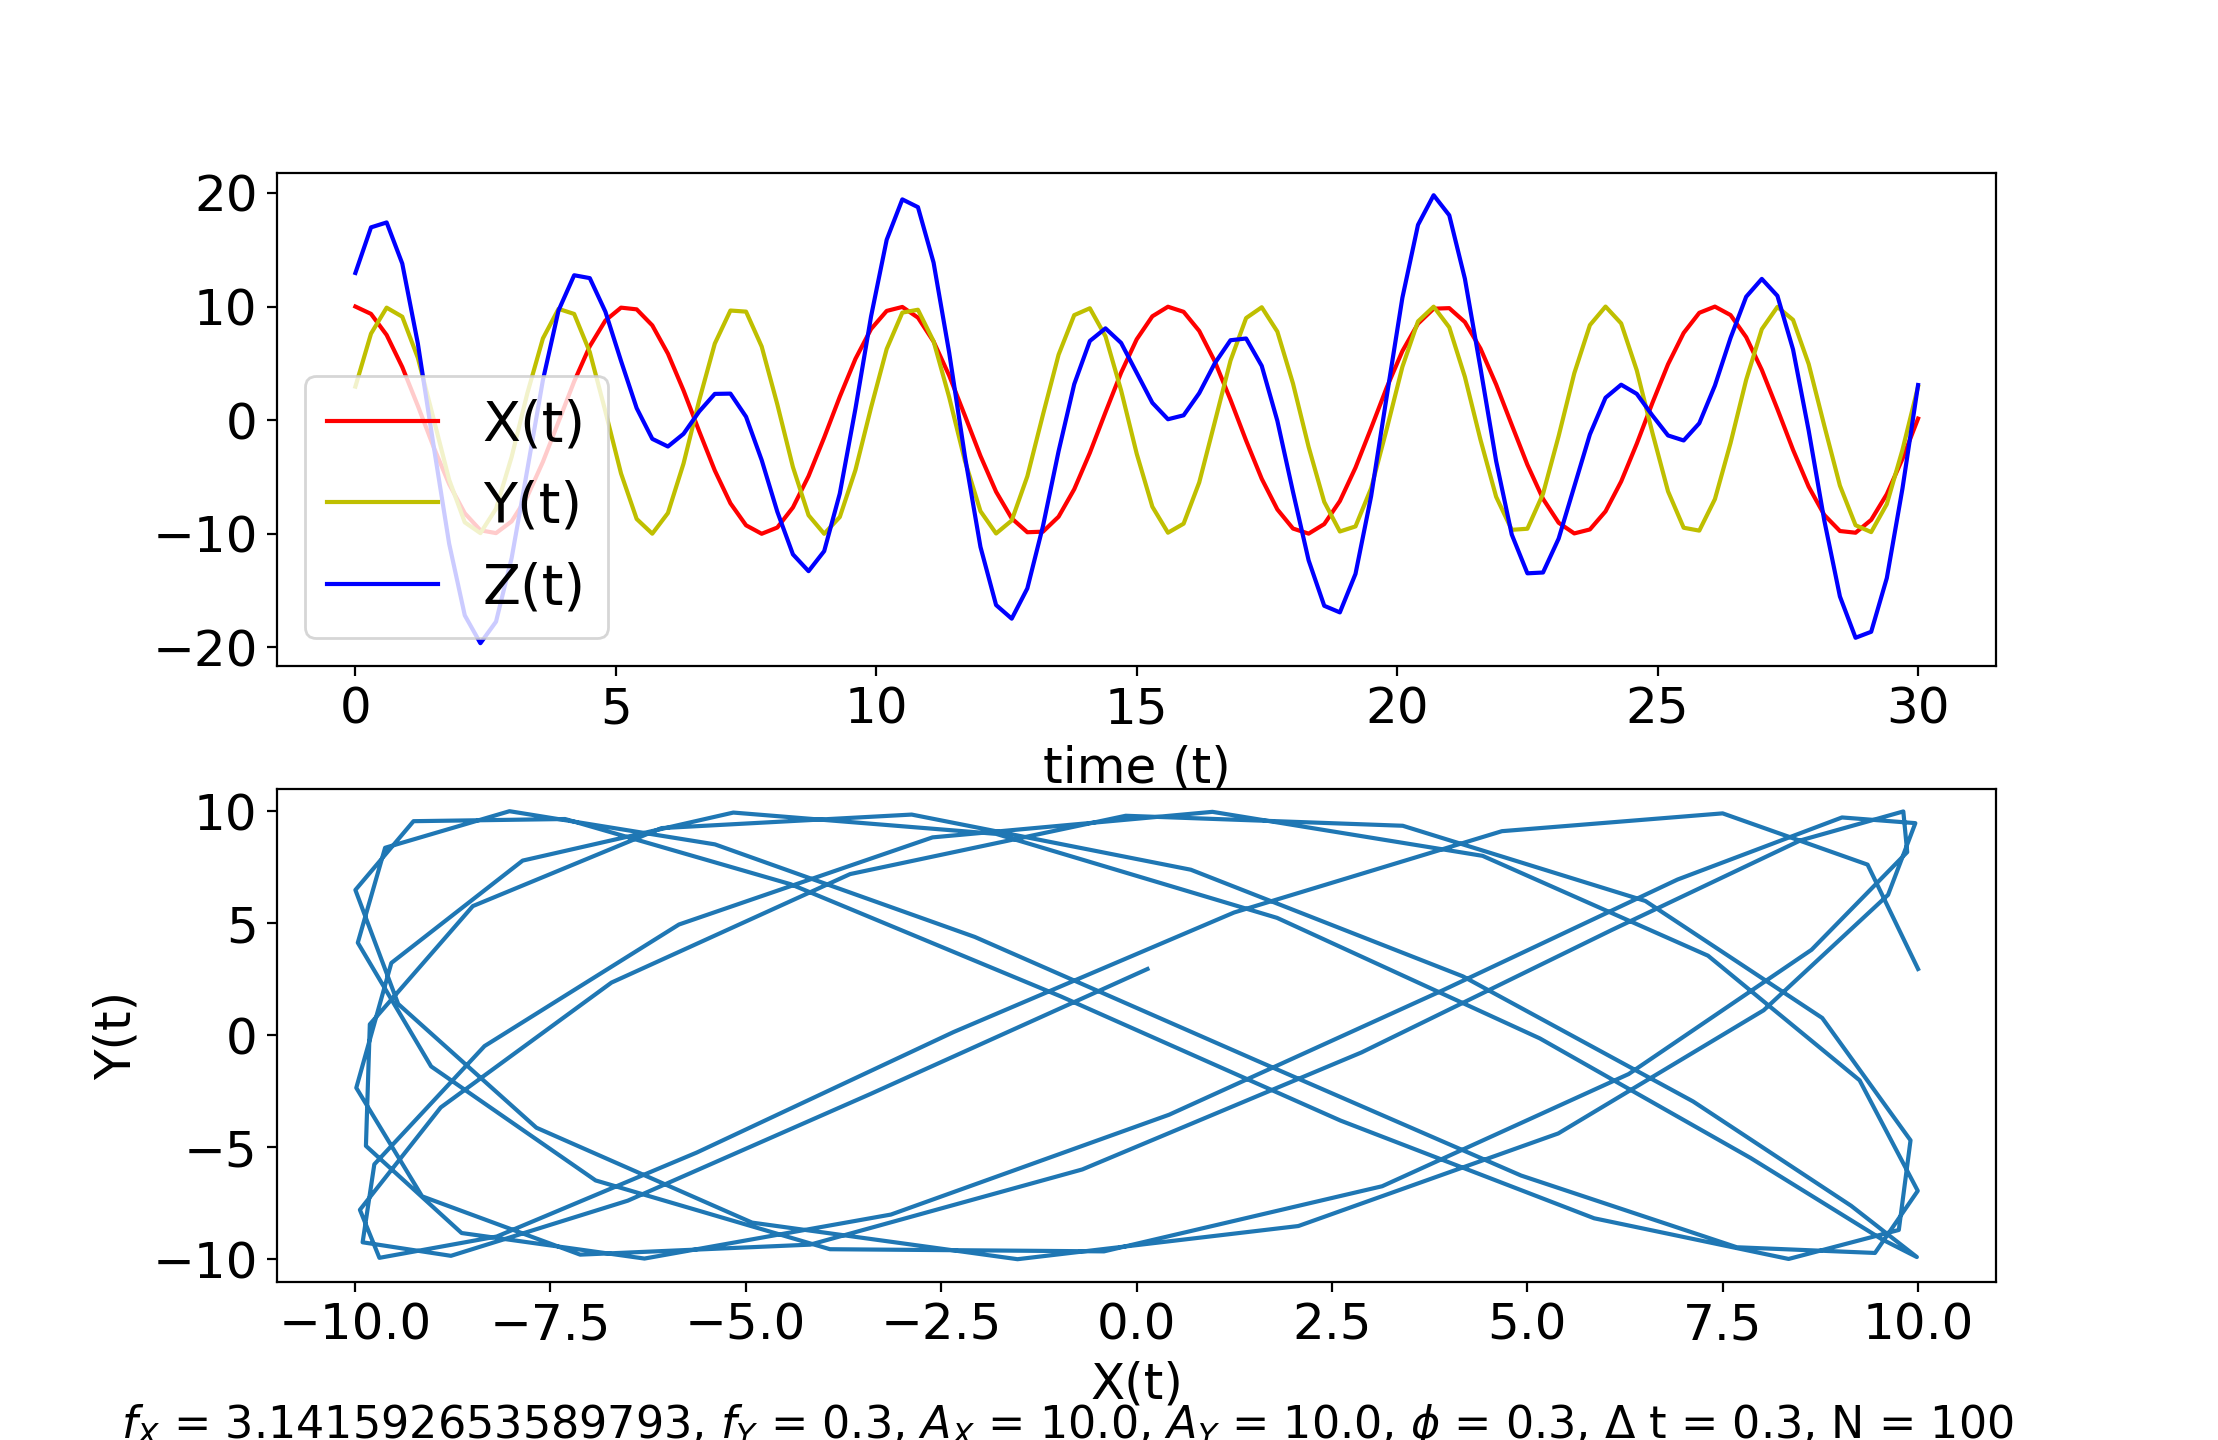
\includegraphics[width=0.48\textwidth]{pi3a.png}}
			\hspace{2mm}
			\subfloat[$\frac{f_X}{f_Y} = 0.75$]{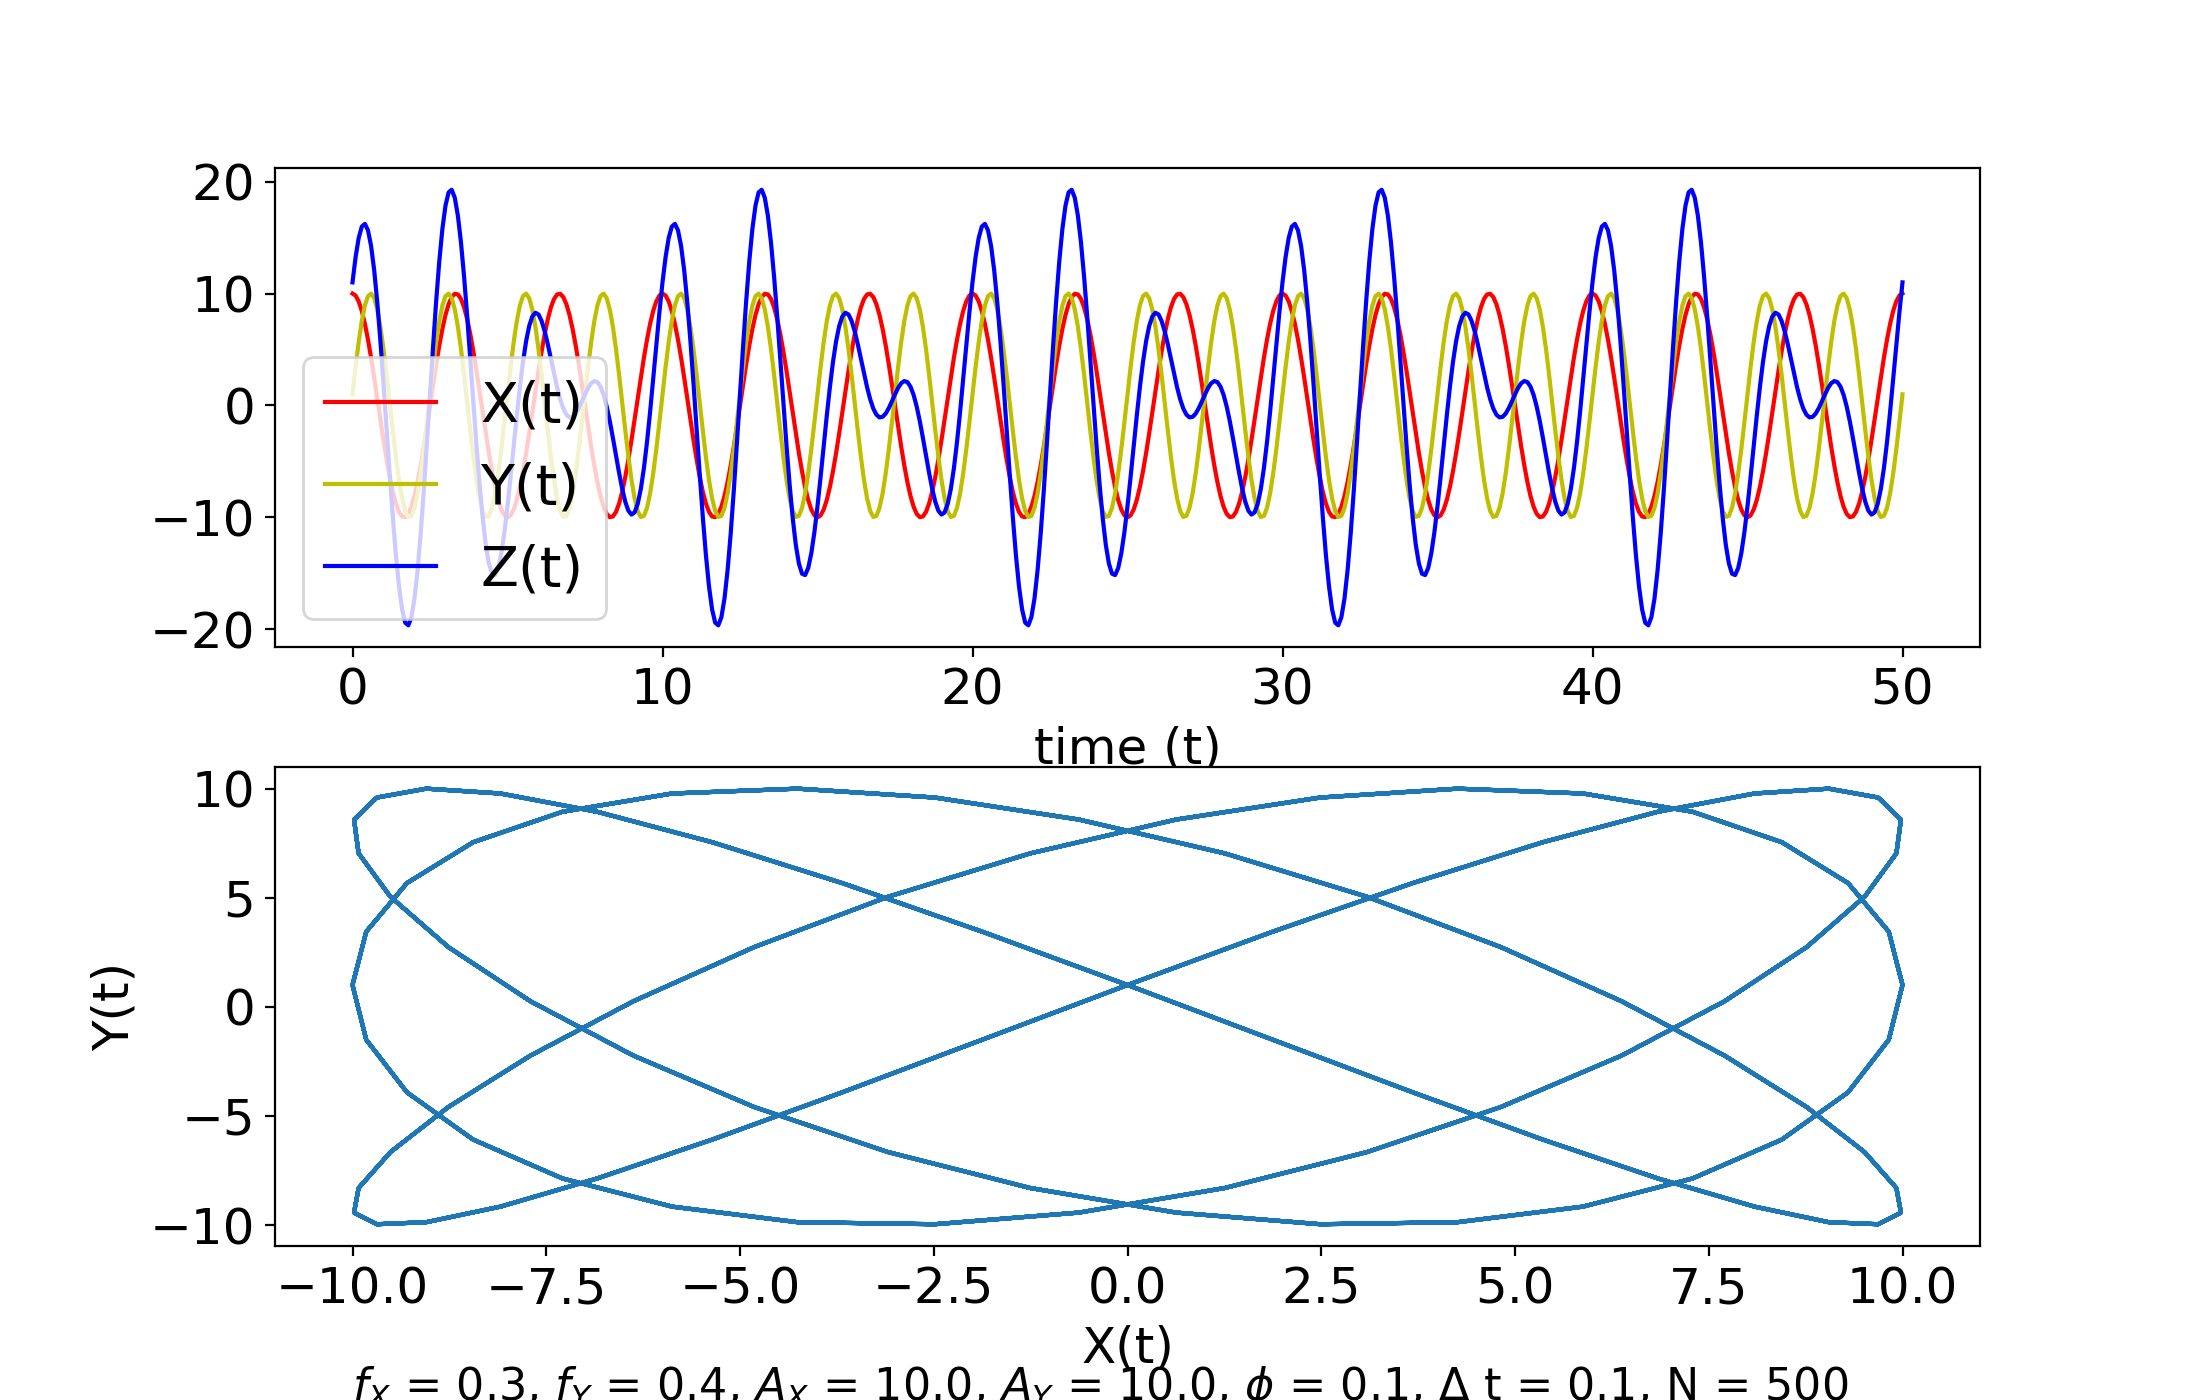
\includegraphics[width=0.48\textwidth]{3aRational1.png}}
			\subfloat[$\frac{f_X}{f_Y} =0.32$]{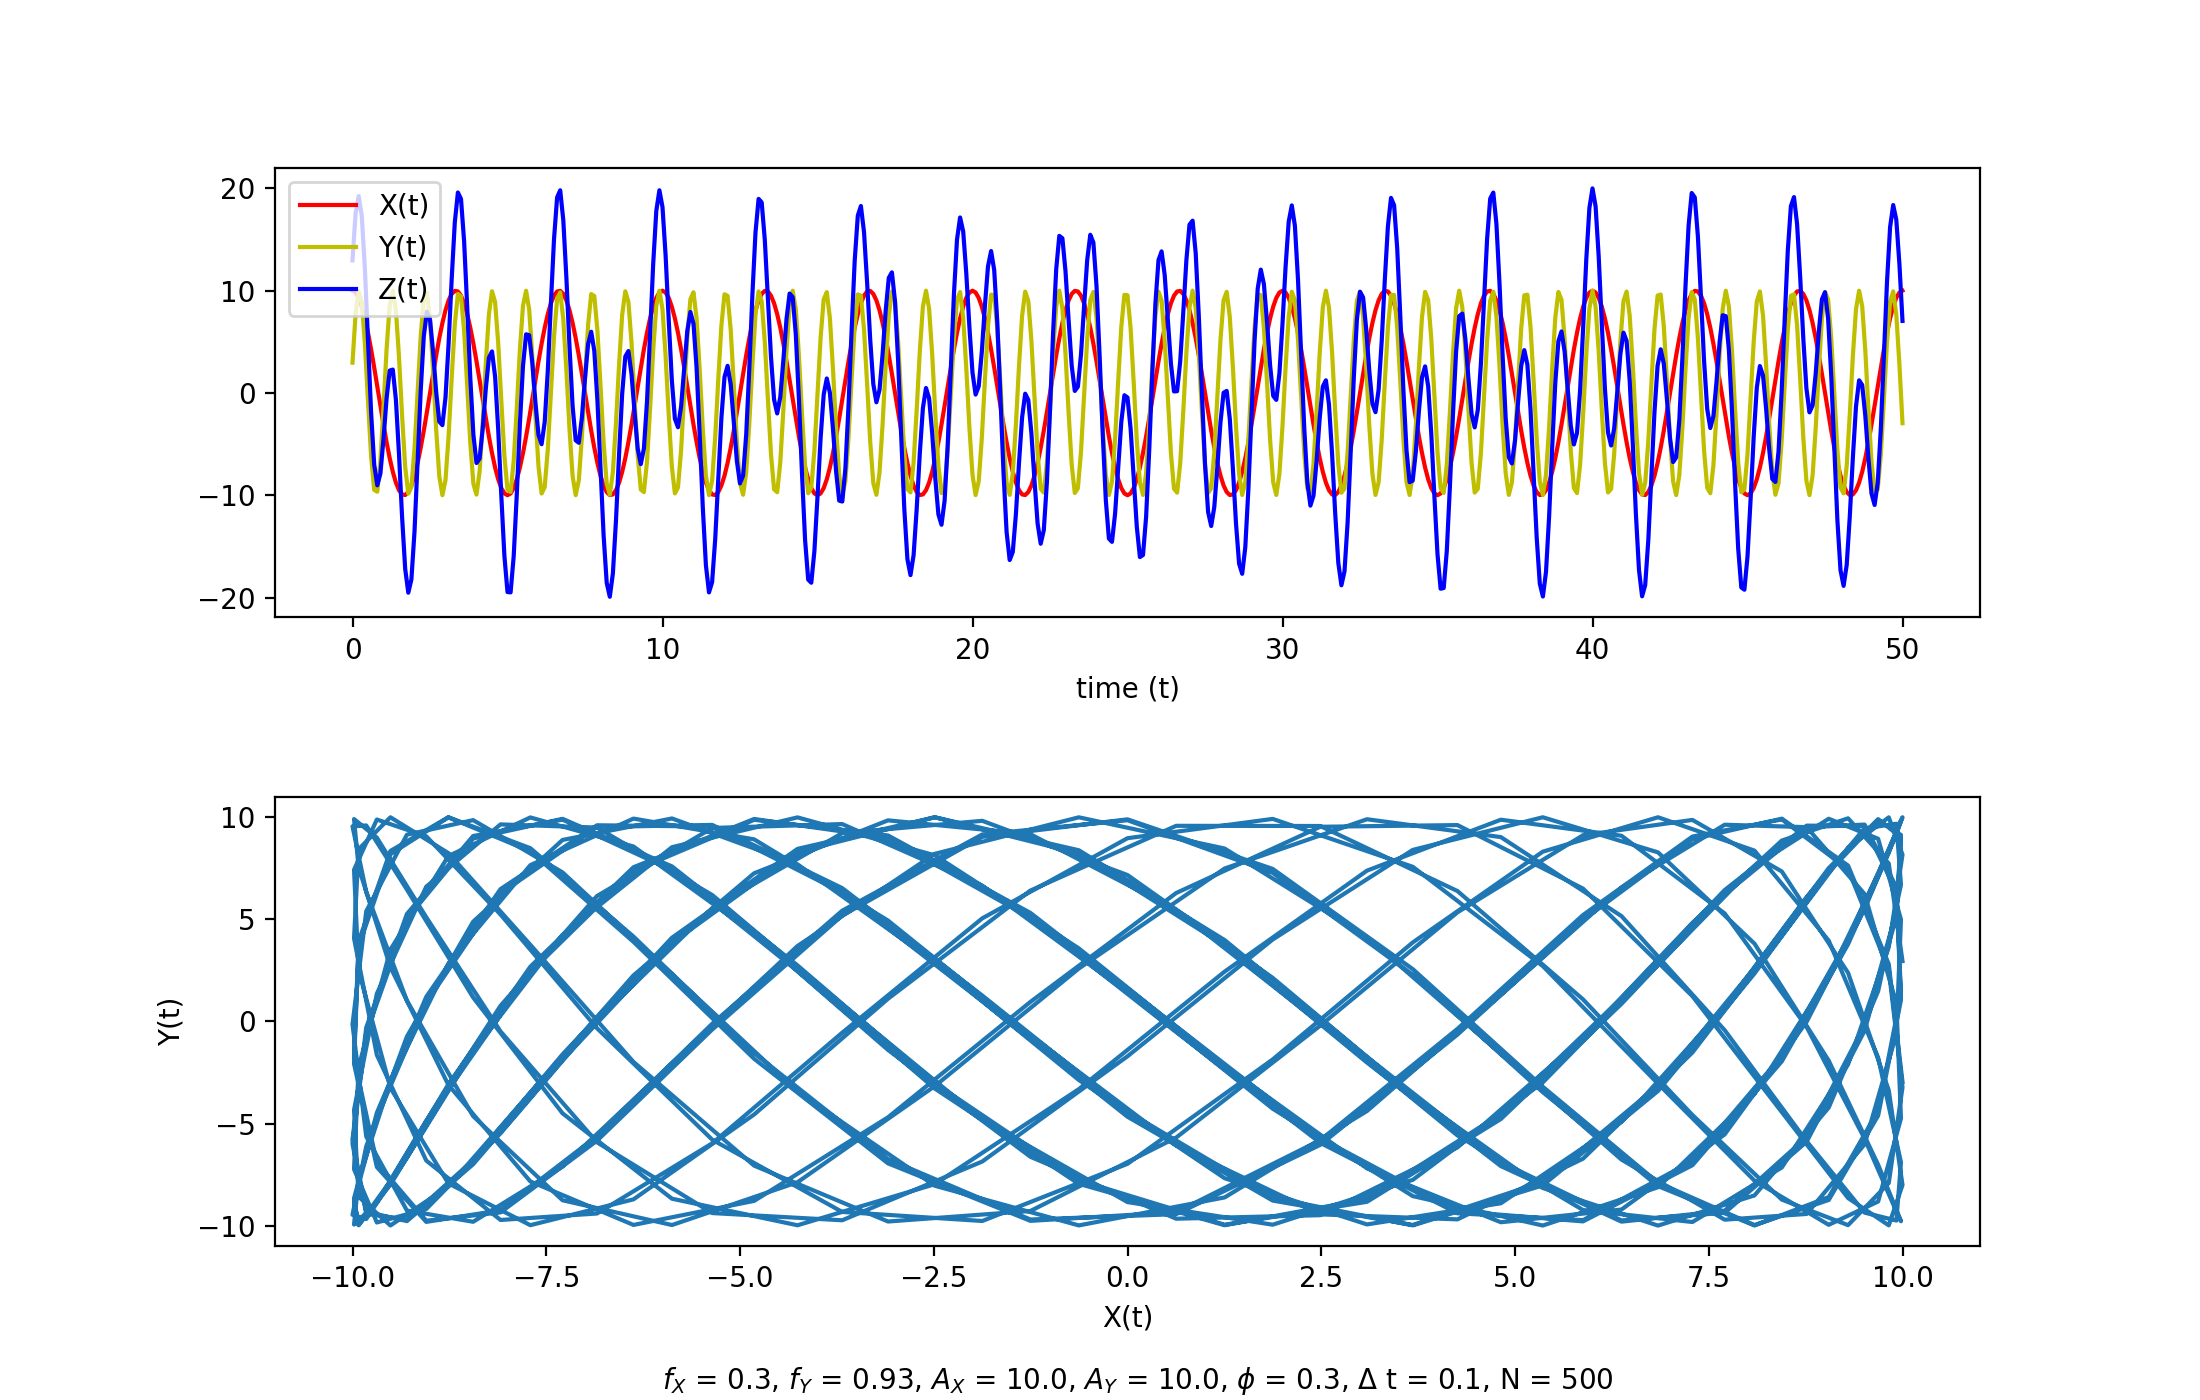
\includegraphics[width=0.48\textwidth]{3aRational2.png}}
			\caption{$\frac{f_X}{f_Y}$ is irrational for (a) and (b) and rational for (c) and (d). (a) and (b) are not closed curves while (c) and (d) are.}\label{fig:3a}
		\end{figure}
		 
		\newpage 
		 
		\indent\textbf{\large b)}
		\begin{figure}[ht]
			\centering
			\subfloat[$\frac{f_X}{f_Y} = 1$]{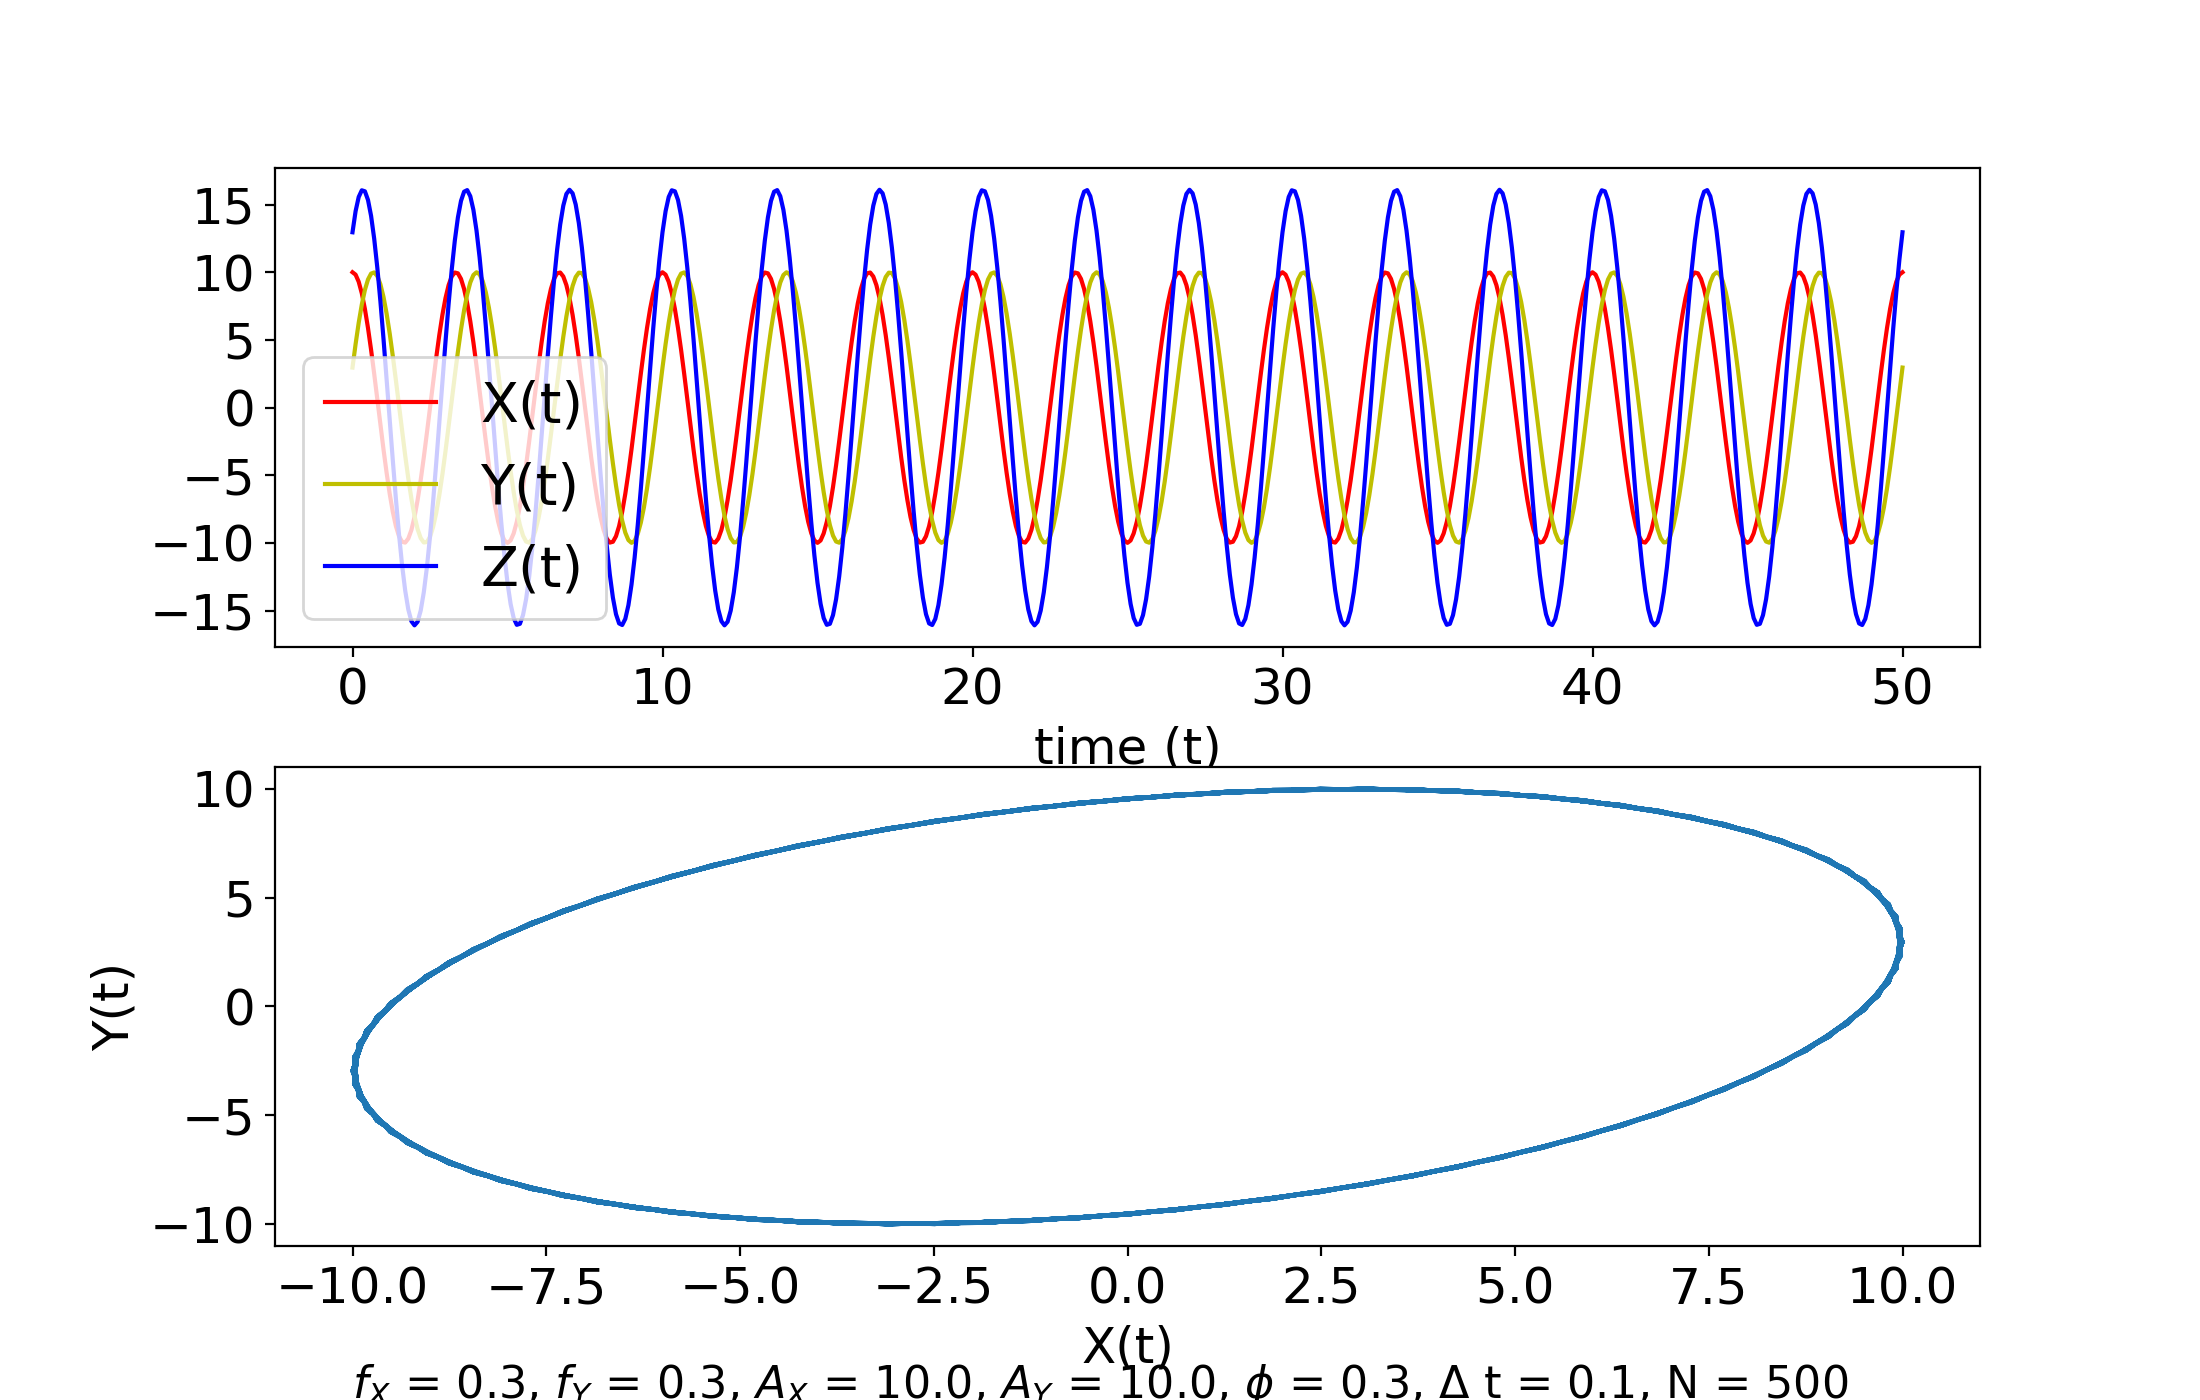
\includegraphics[width=0.48\textwidth]{3b1.png}}
			\subfloat[$\frac{f_X}{f_Y} = \frac{1}{2}$]{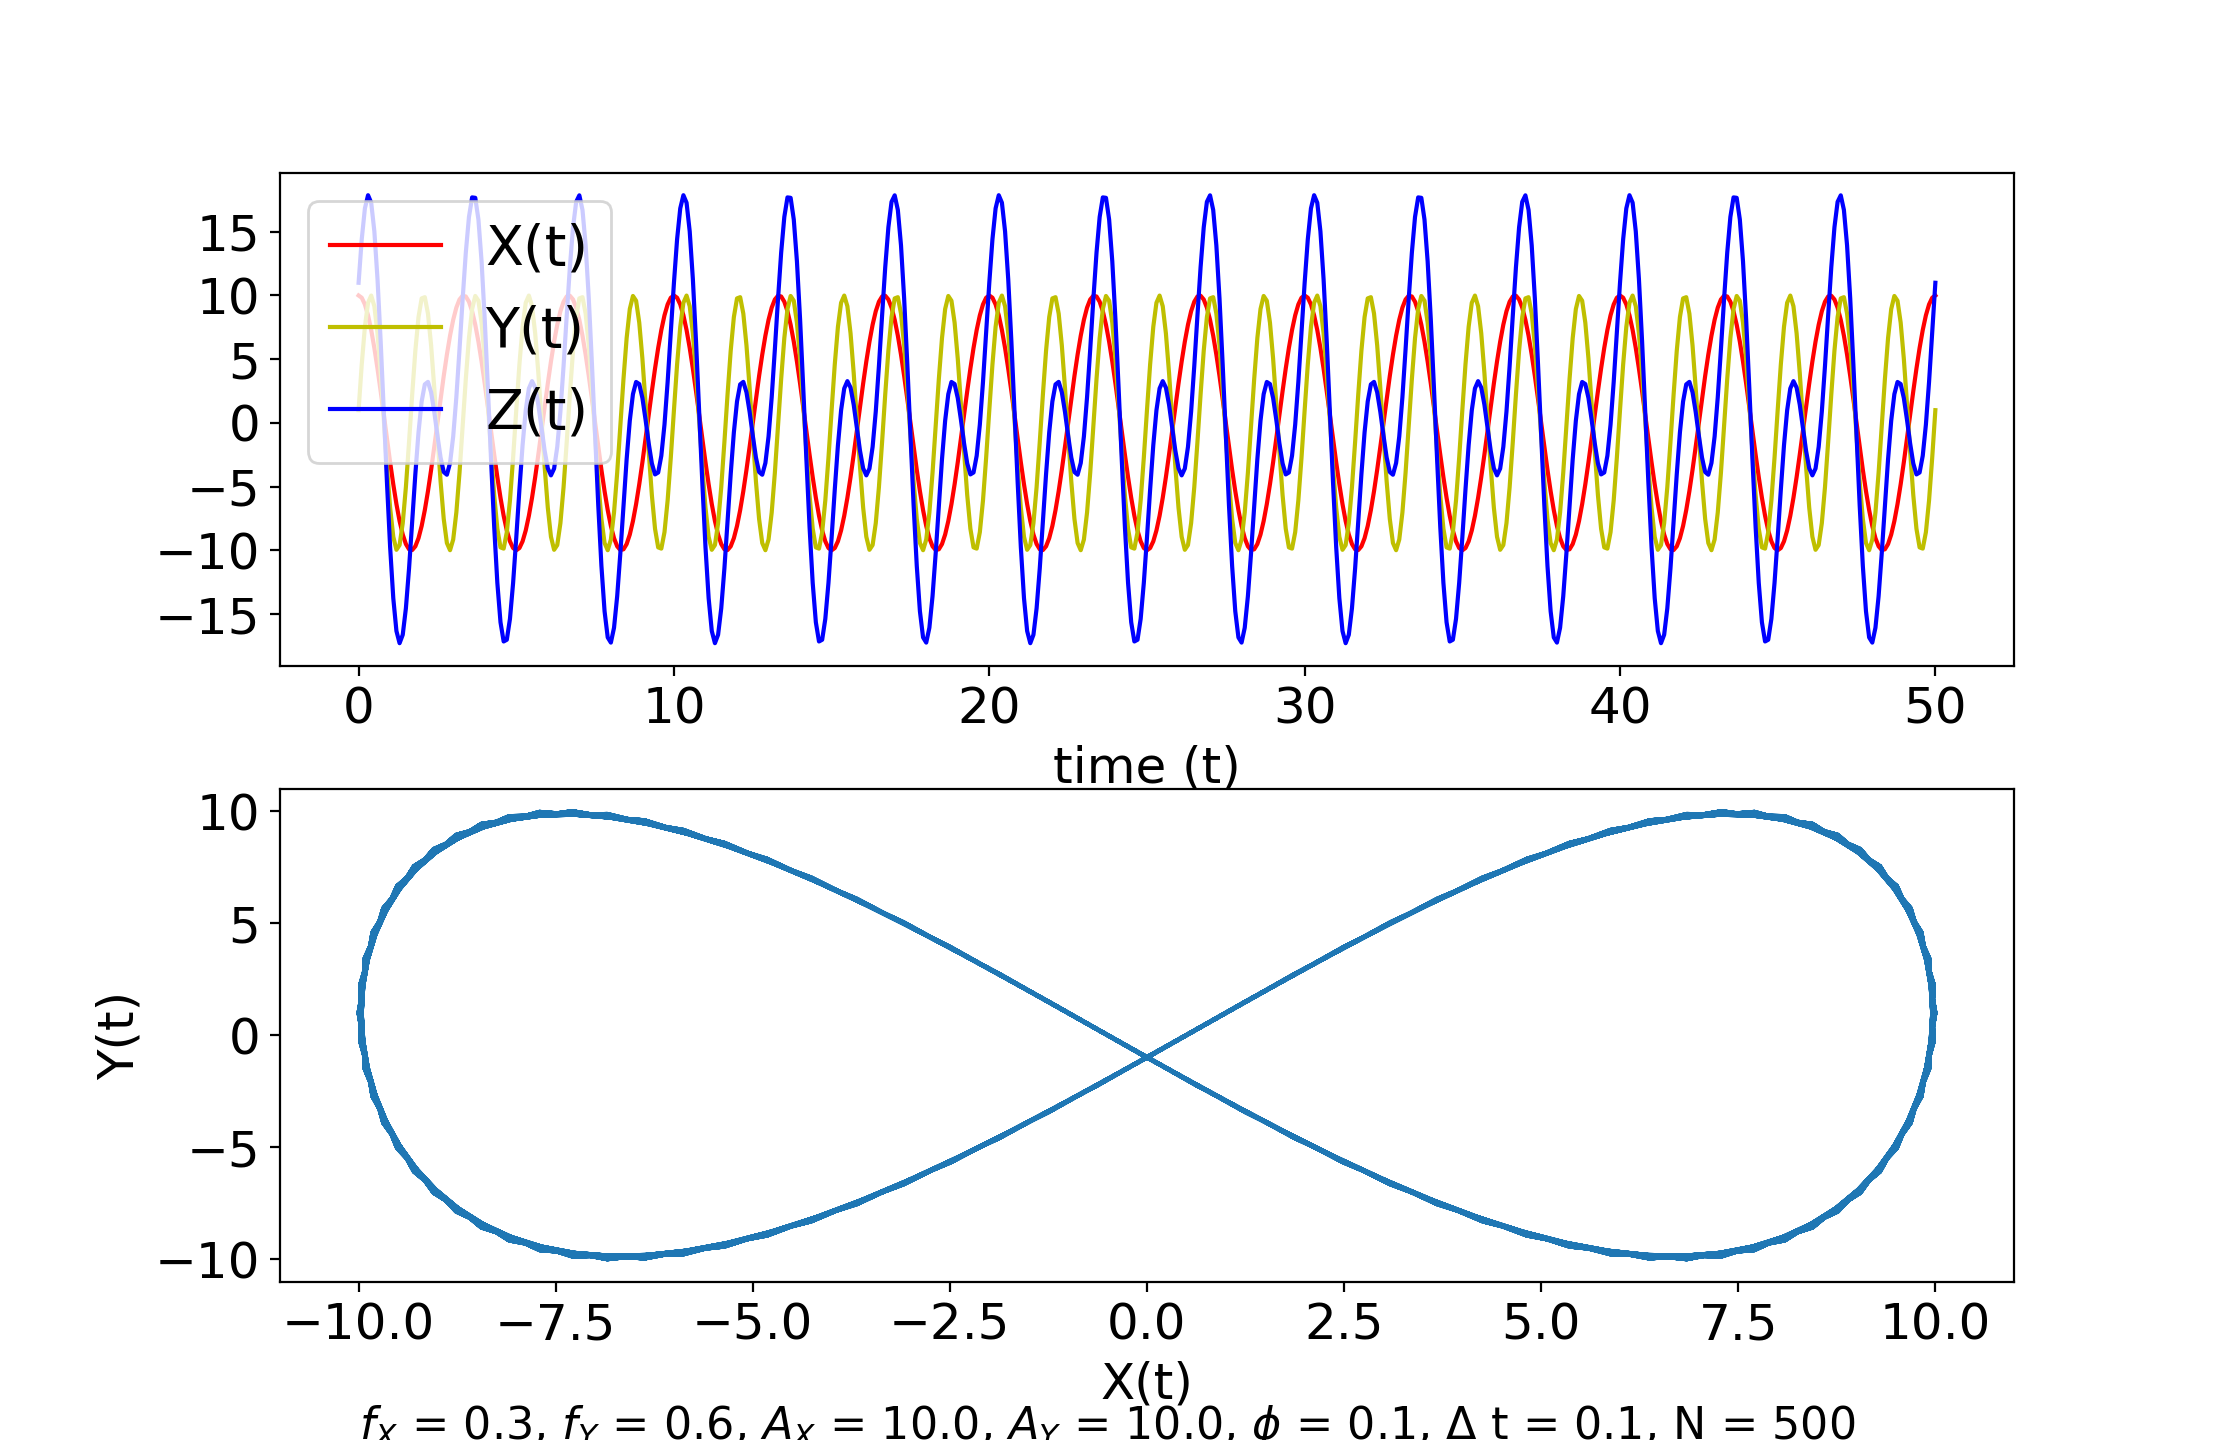
\includegraphics[width=0.48\textwidth]{3b2.png}}
			\hspace{2mm}
			\subfloat[$\frac{f_X}{f_Y} = \frac{1}{3}$]{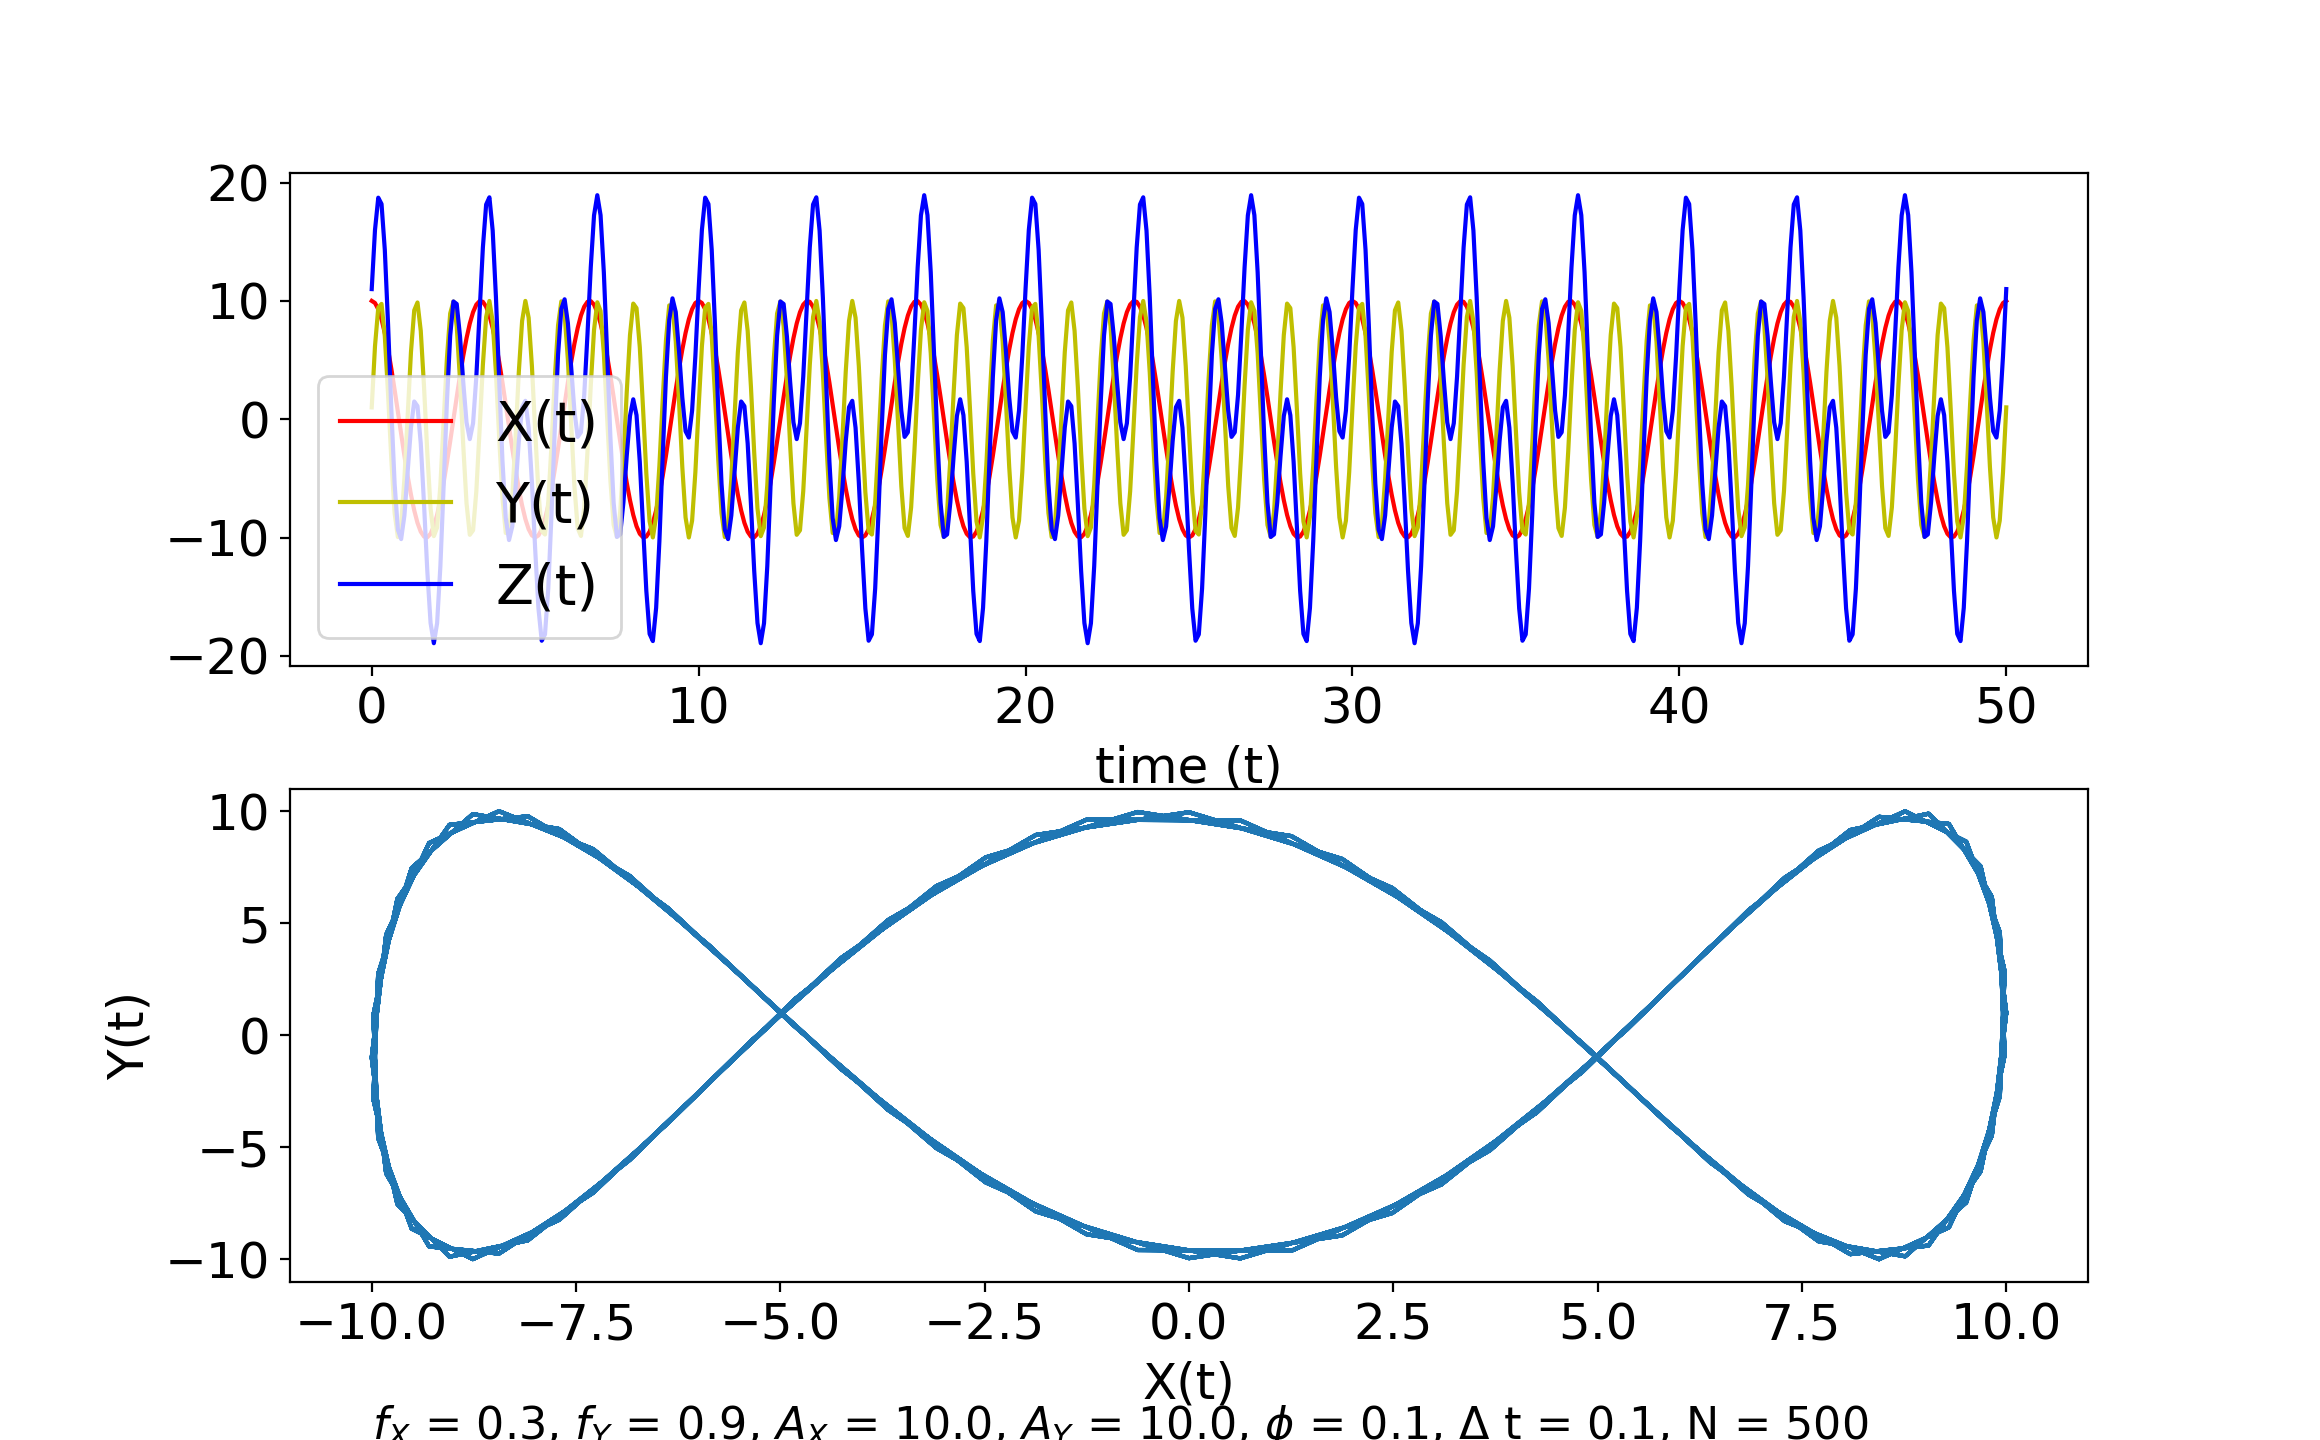
\includegraphics[width=0.48\textwidth]{3b4.png}}
			\subfloat[$\frac{f_X}{f_Y} = \frac{1}{4}$]{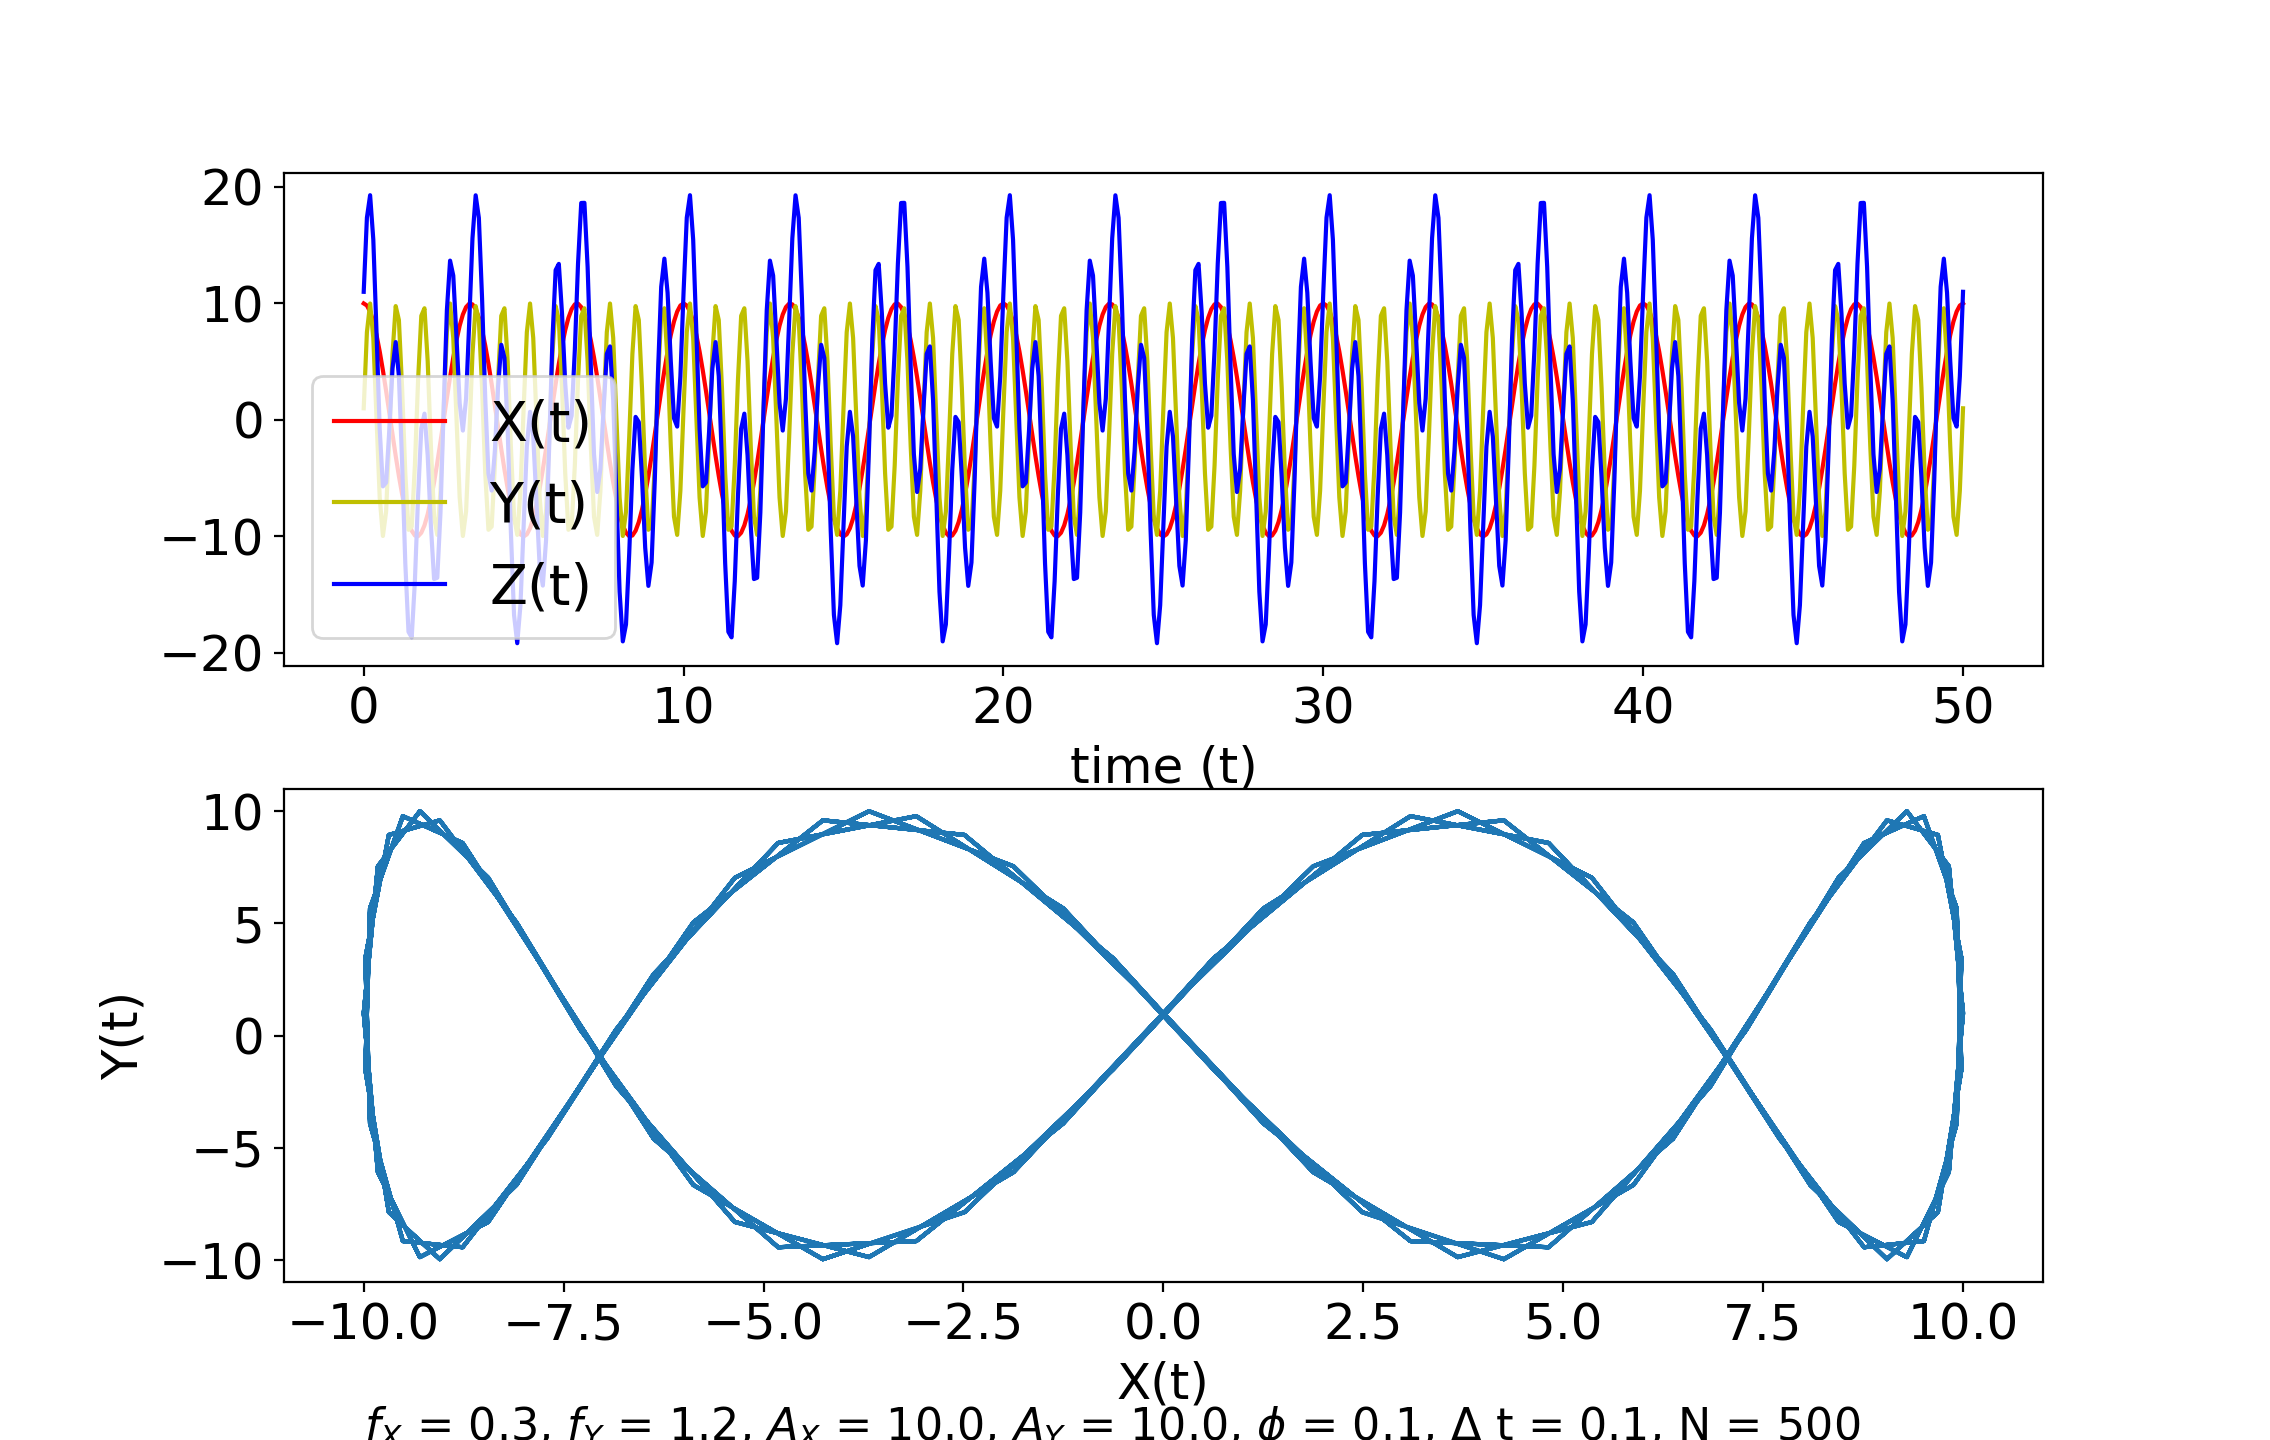
\includegraphics[width=0.48\textwidth]{3b5.png}}
			\caption{$\frac{f_X}{f_Y}$ determines the number of intersections of the $X(t)$ vs $Y(t)$ curve. When $\frac{1}{f_X / f_Y}$ is a natural number, $\frac{1}{f_X / f_Y}$ is the number of sections the curve is divided into.}\label{fig:3b}
		\end{figure}
	
		\indent\textbf{\large c)}
		\begin{figure}[H]
			\centering
			\subfloat[$\phi = 0$]{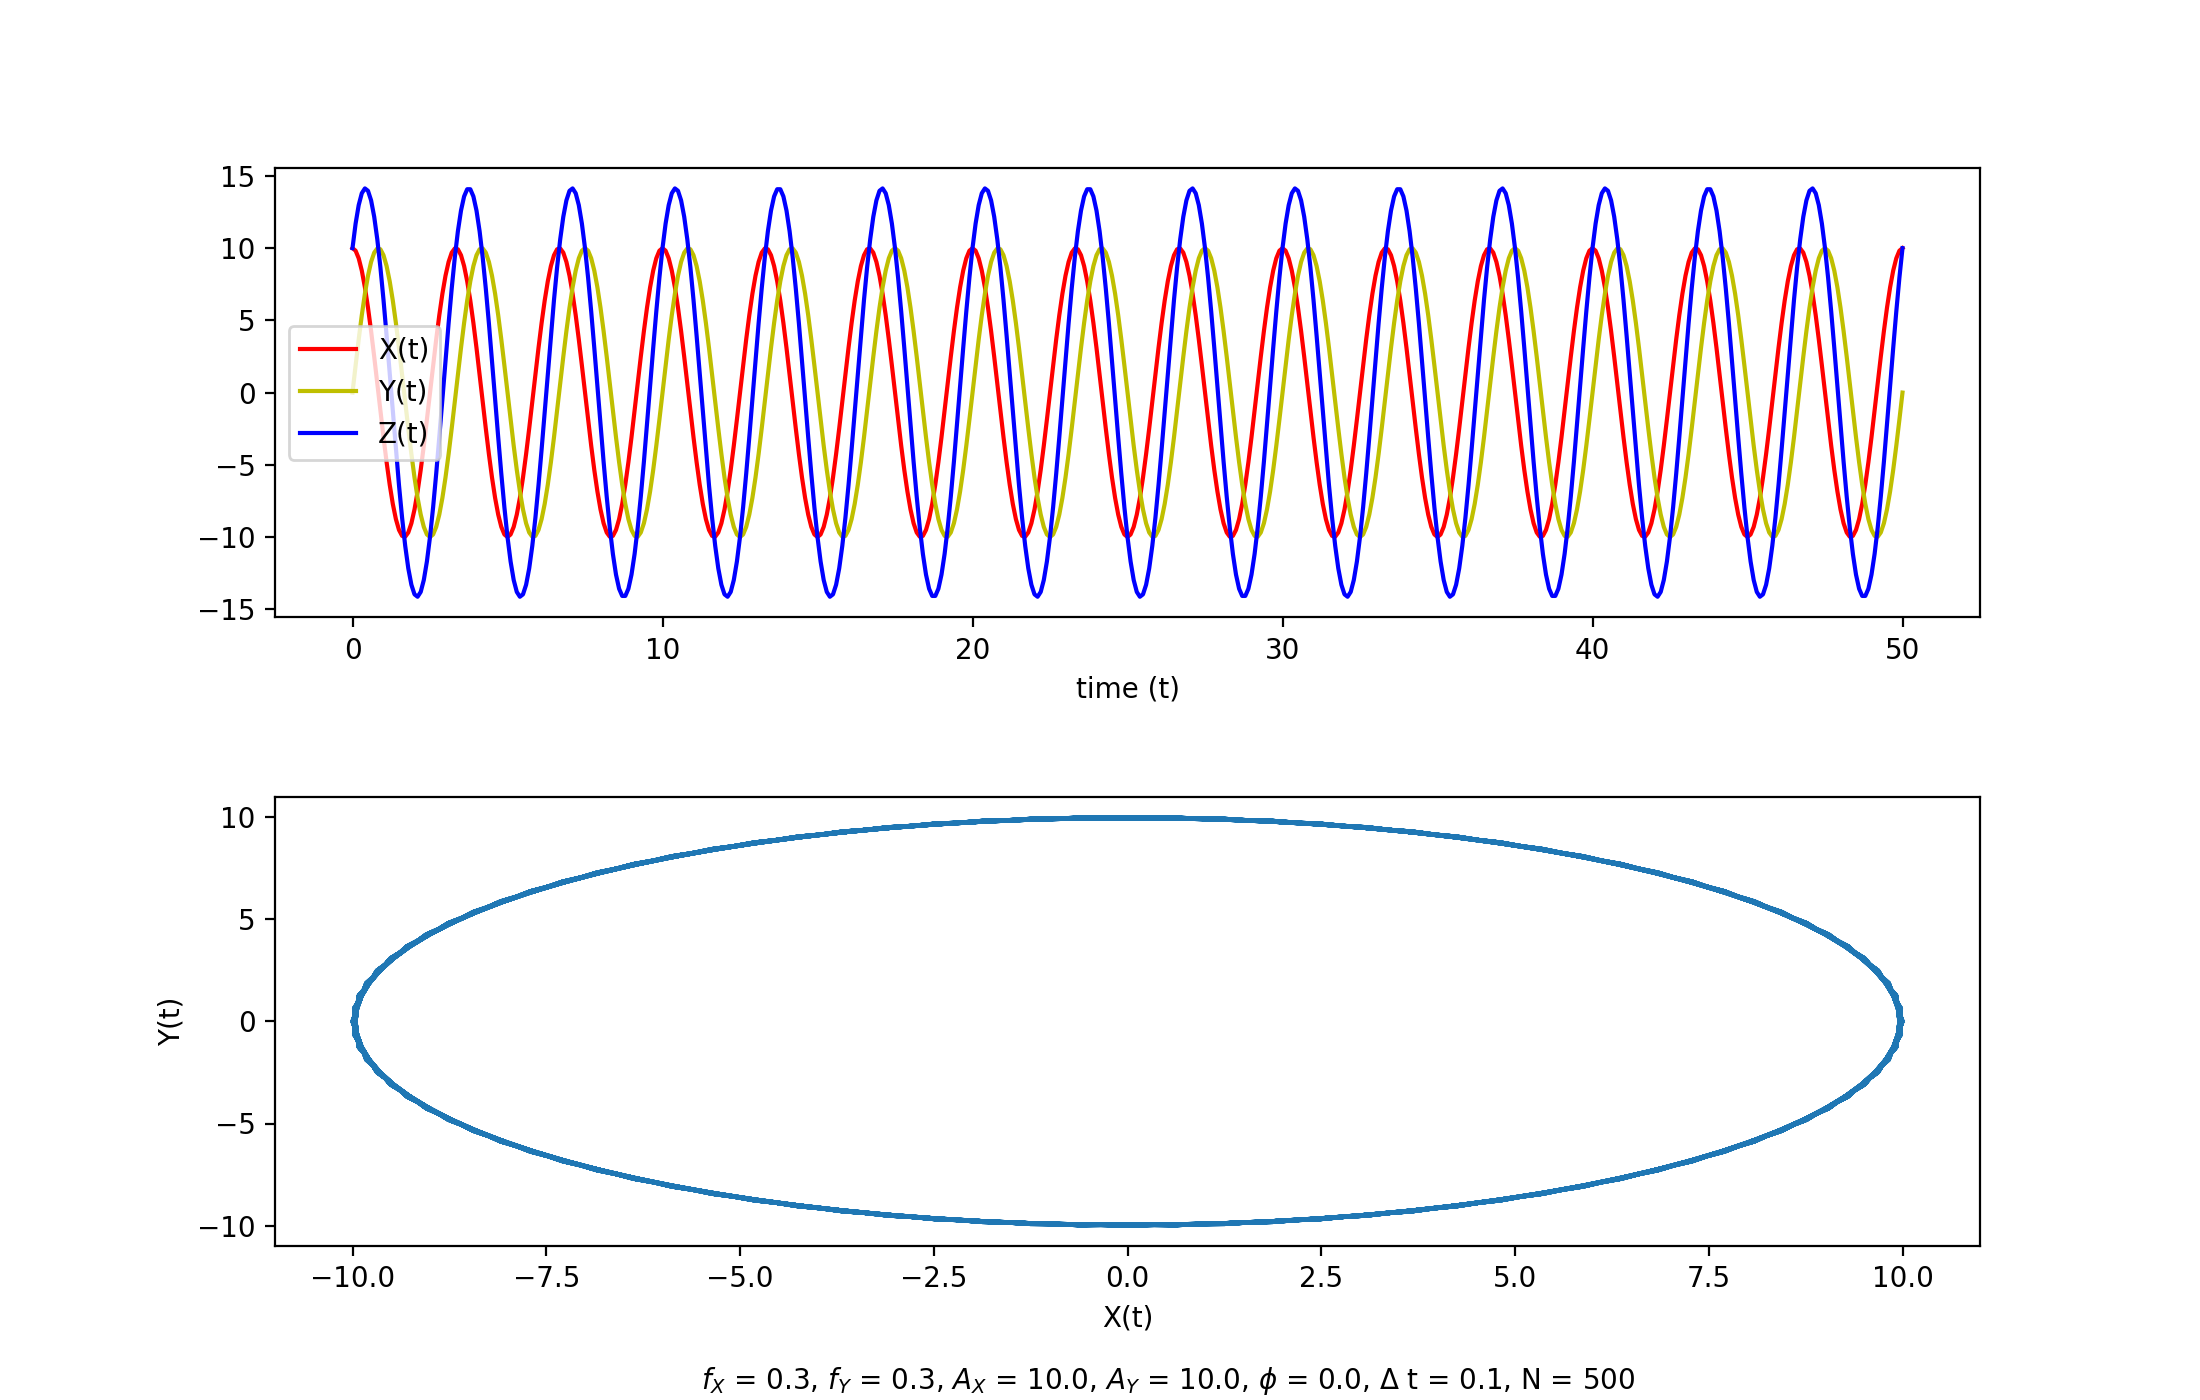
\includegraphics[width=0.48\textwidth]{3c1.png}}
			\subfloat[$\phi = \frac{\pi}{6}$]{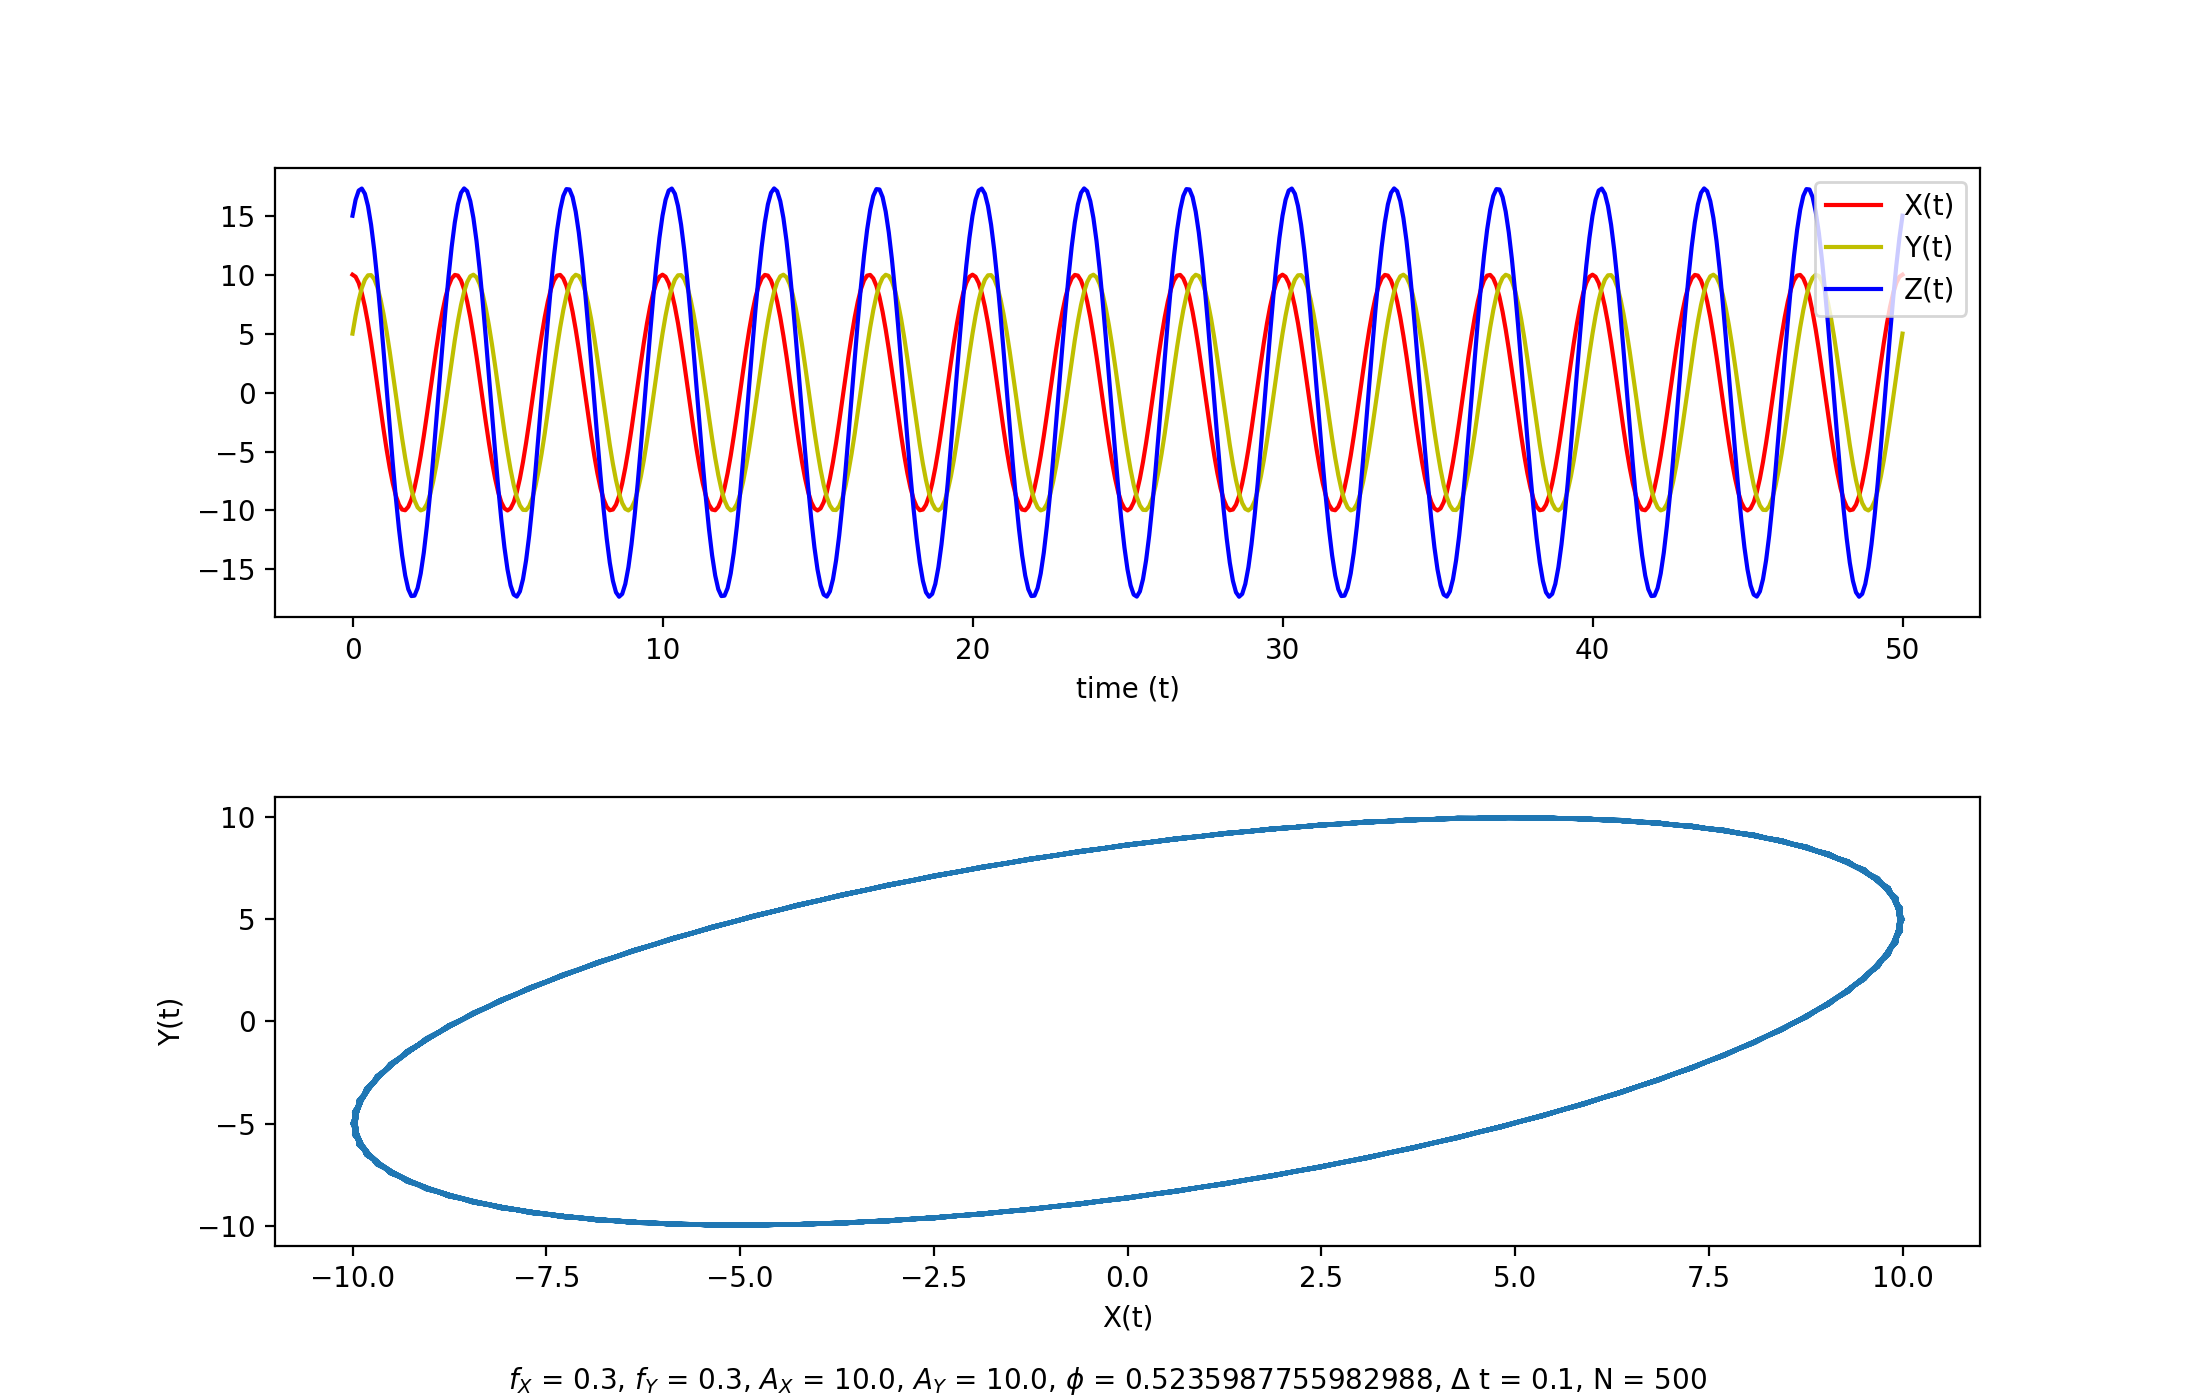
\includegraphics[width=0.48\textwidth]{3c2.png}}
		\end{figure}
		\begin{figure}[ht]
			\renewcommand{\thesubfigure}{c}
			\subfloat[$\phi = \frac{\pi}{4}$]{\label{first}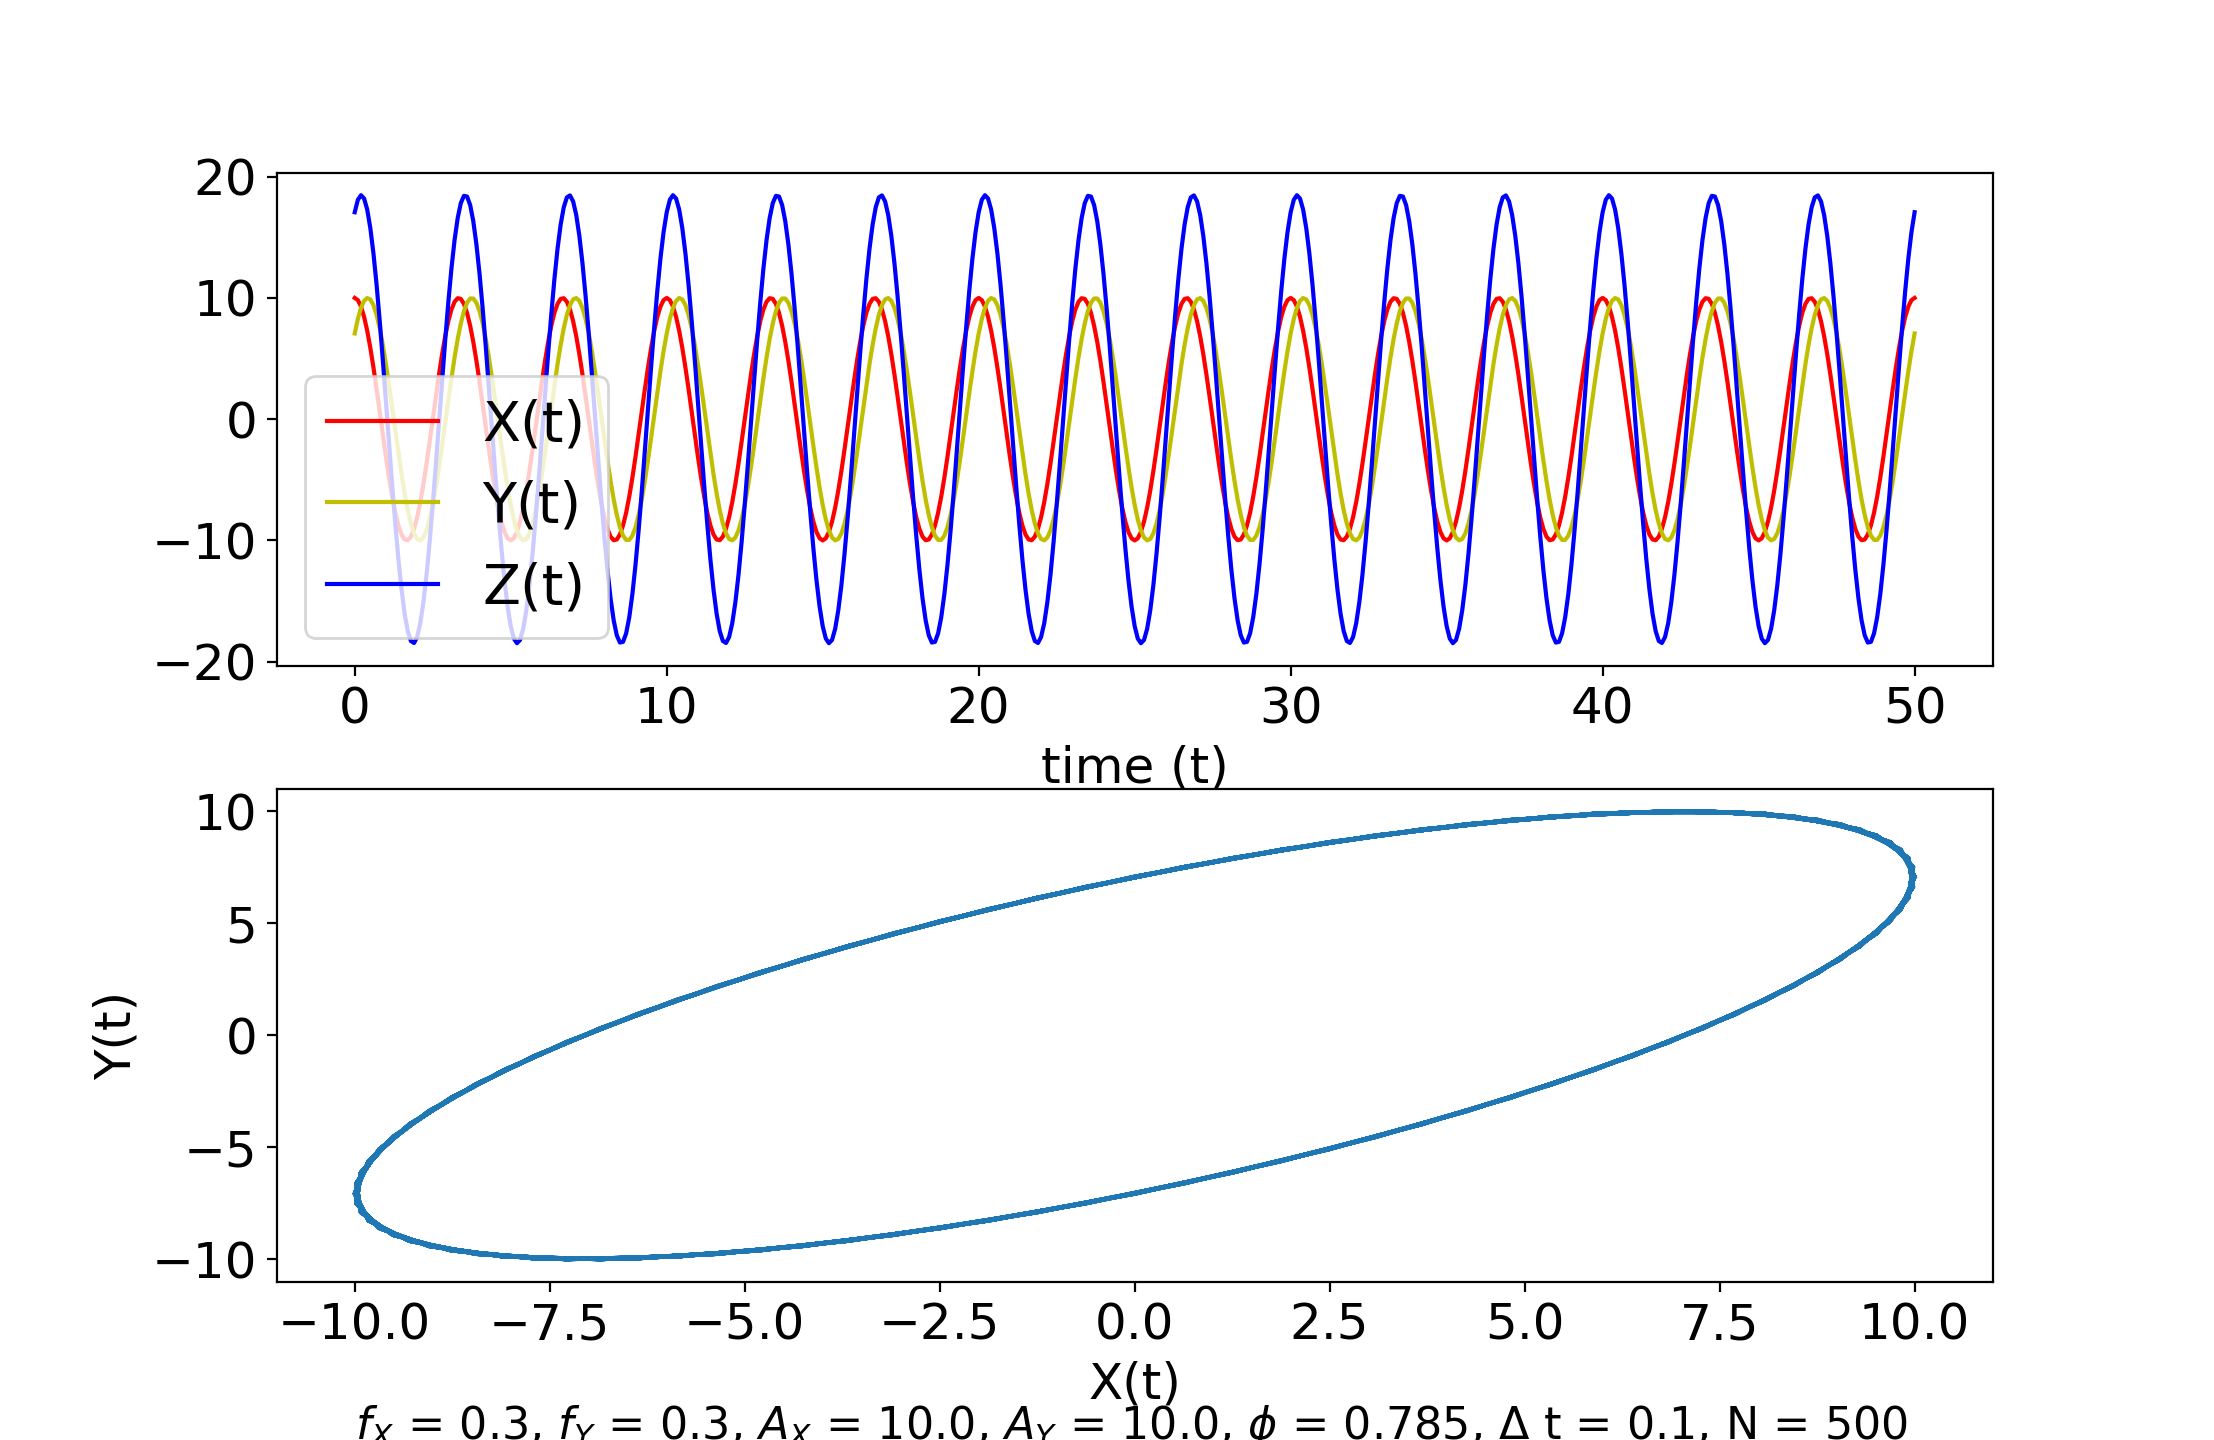
\includegraphics[width=0.48\textwidth]{3c3.png}}
			\renewcommand{\thesubfigure}{d}
			\subfloat[$\phi = \frac{\pi}{2}$]{\label{second}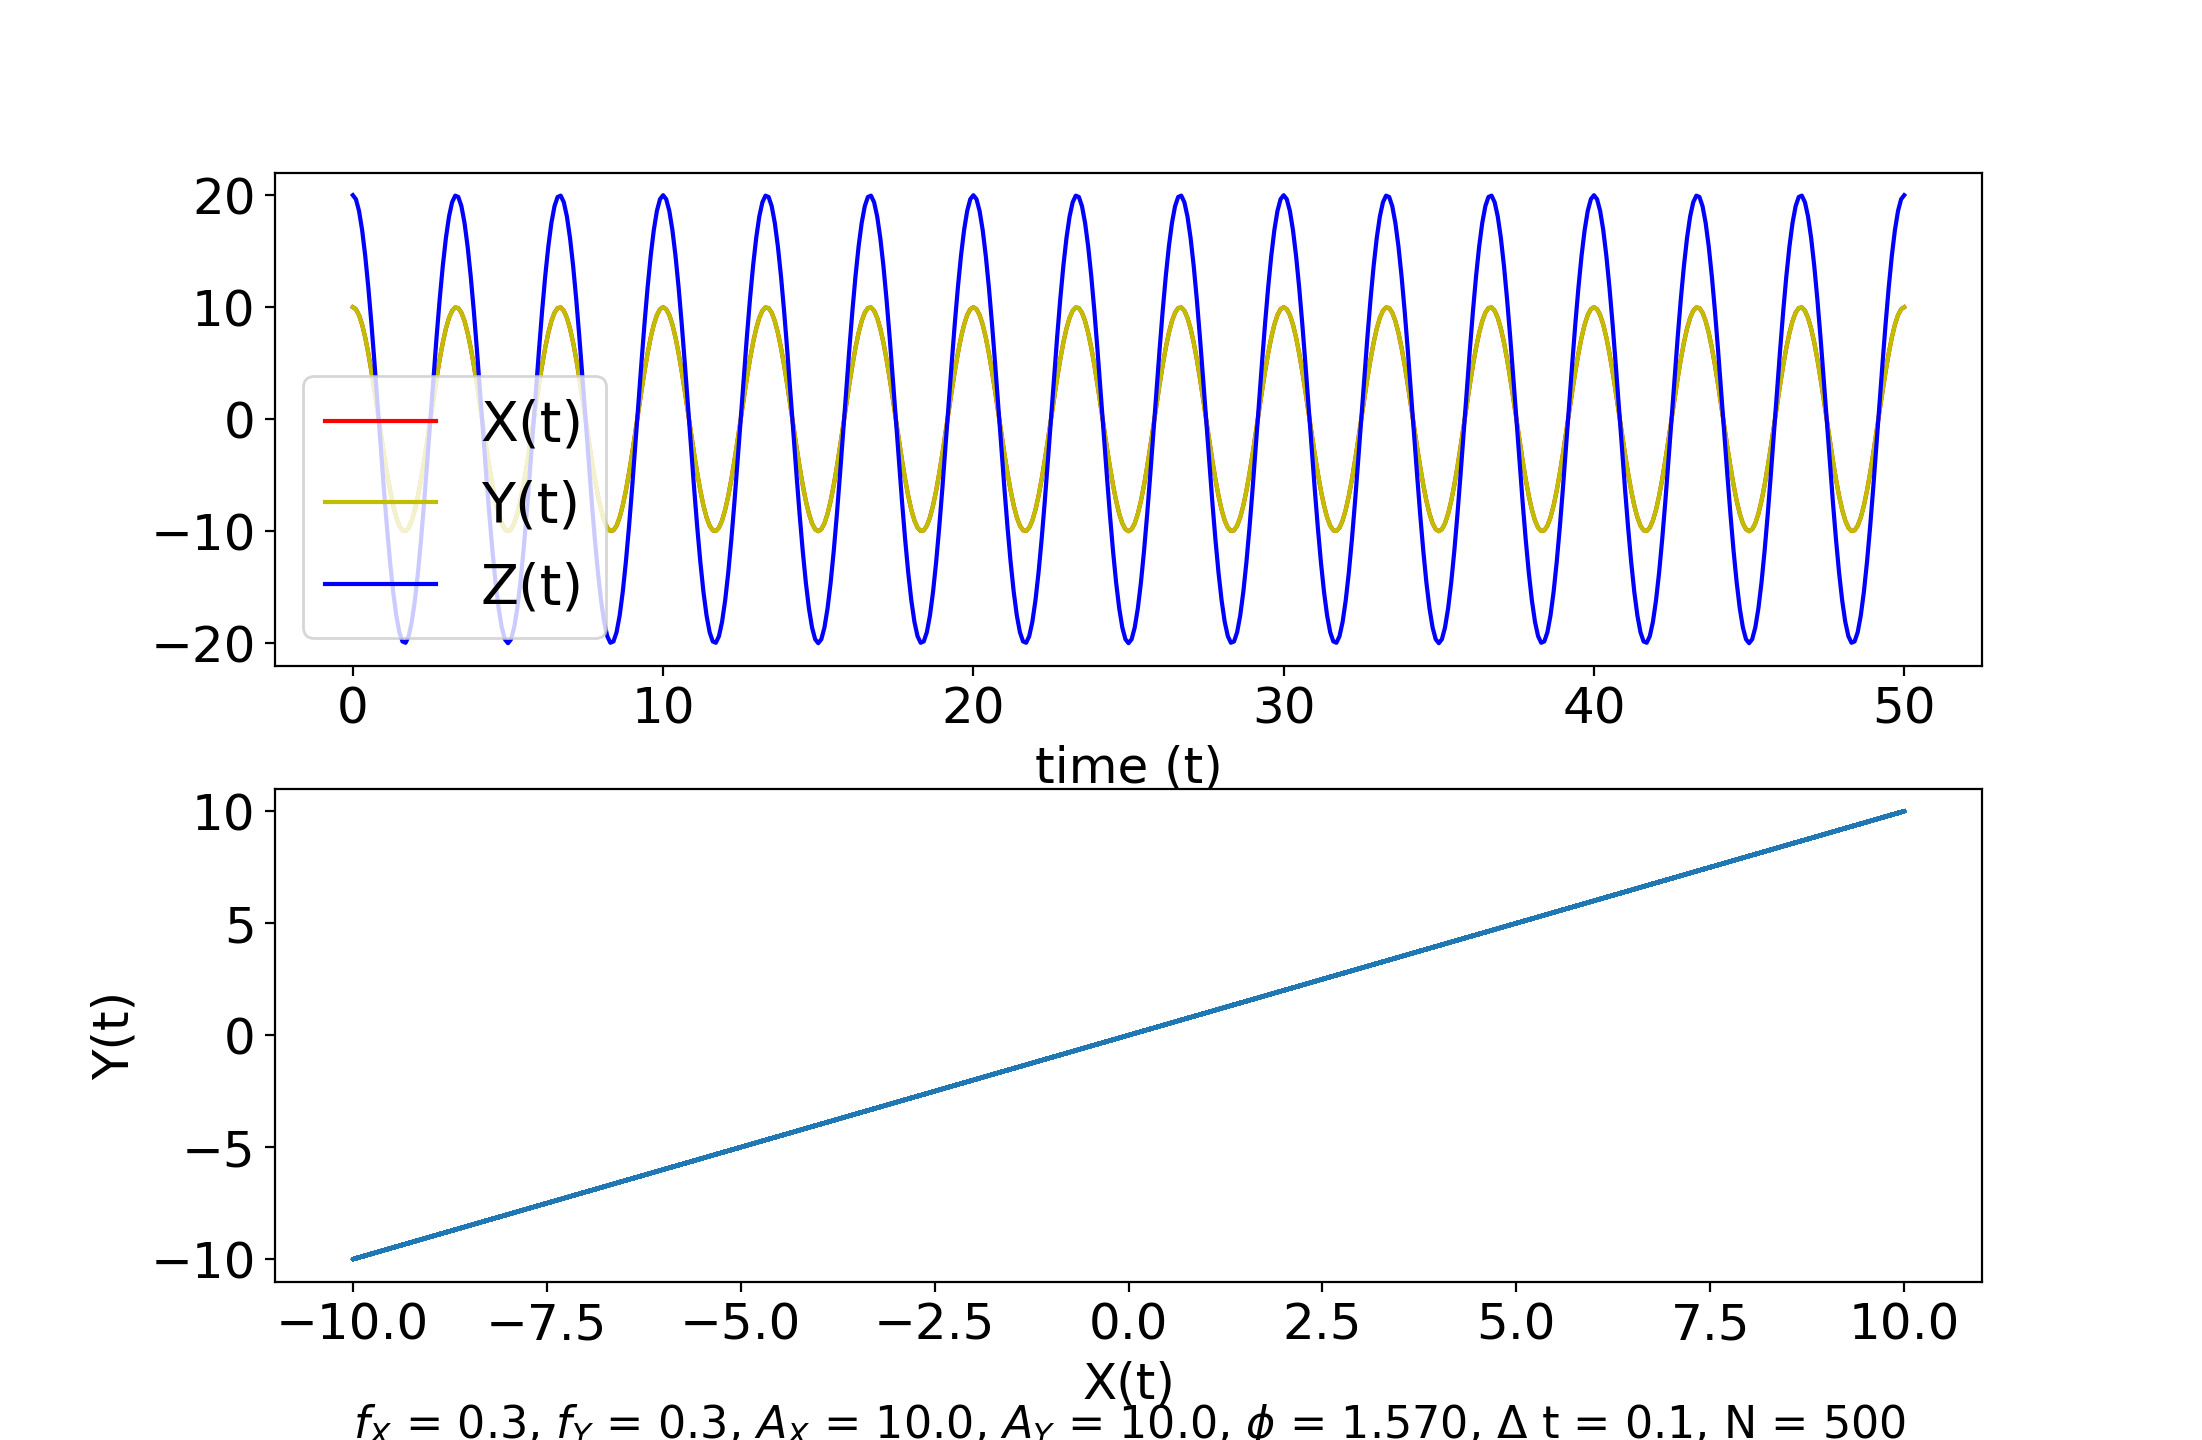
\includegraphics[width=0.48\textwidth]{3c4.png}}
			\caption{When $f_X = f_Y$, $\phi$ affects the apperent rotation angle of the figure.}\label{fig:3c}
		\end{figure}
	
		The plots can show us the phase and frequency differences between electronic circuits. Using an oscilloscope to adjust the phase, one can see that once Lissajous figure is elliptical, the circuits are tuned. When the Lissajous appears to be linear (see Figure~\ref{fig:3c}d), the circuits also have the same phase shift.
	
	\newpage	
		
	\noindent\textbf{\large Problem 4}
	\begin{figure}[ht]
		\subfloat[]{\label{first}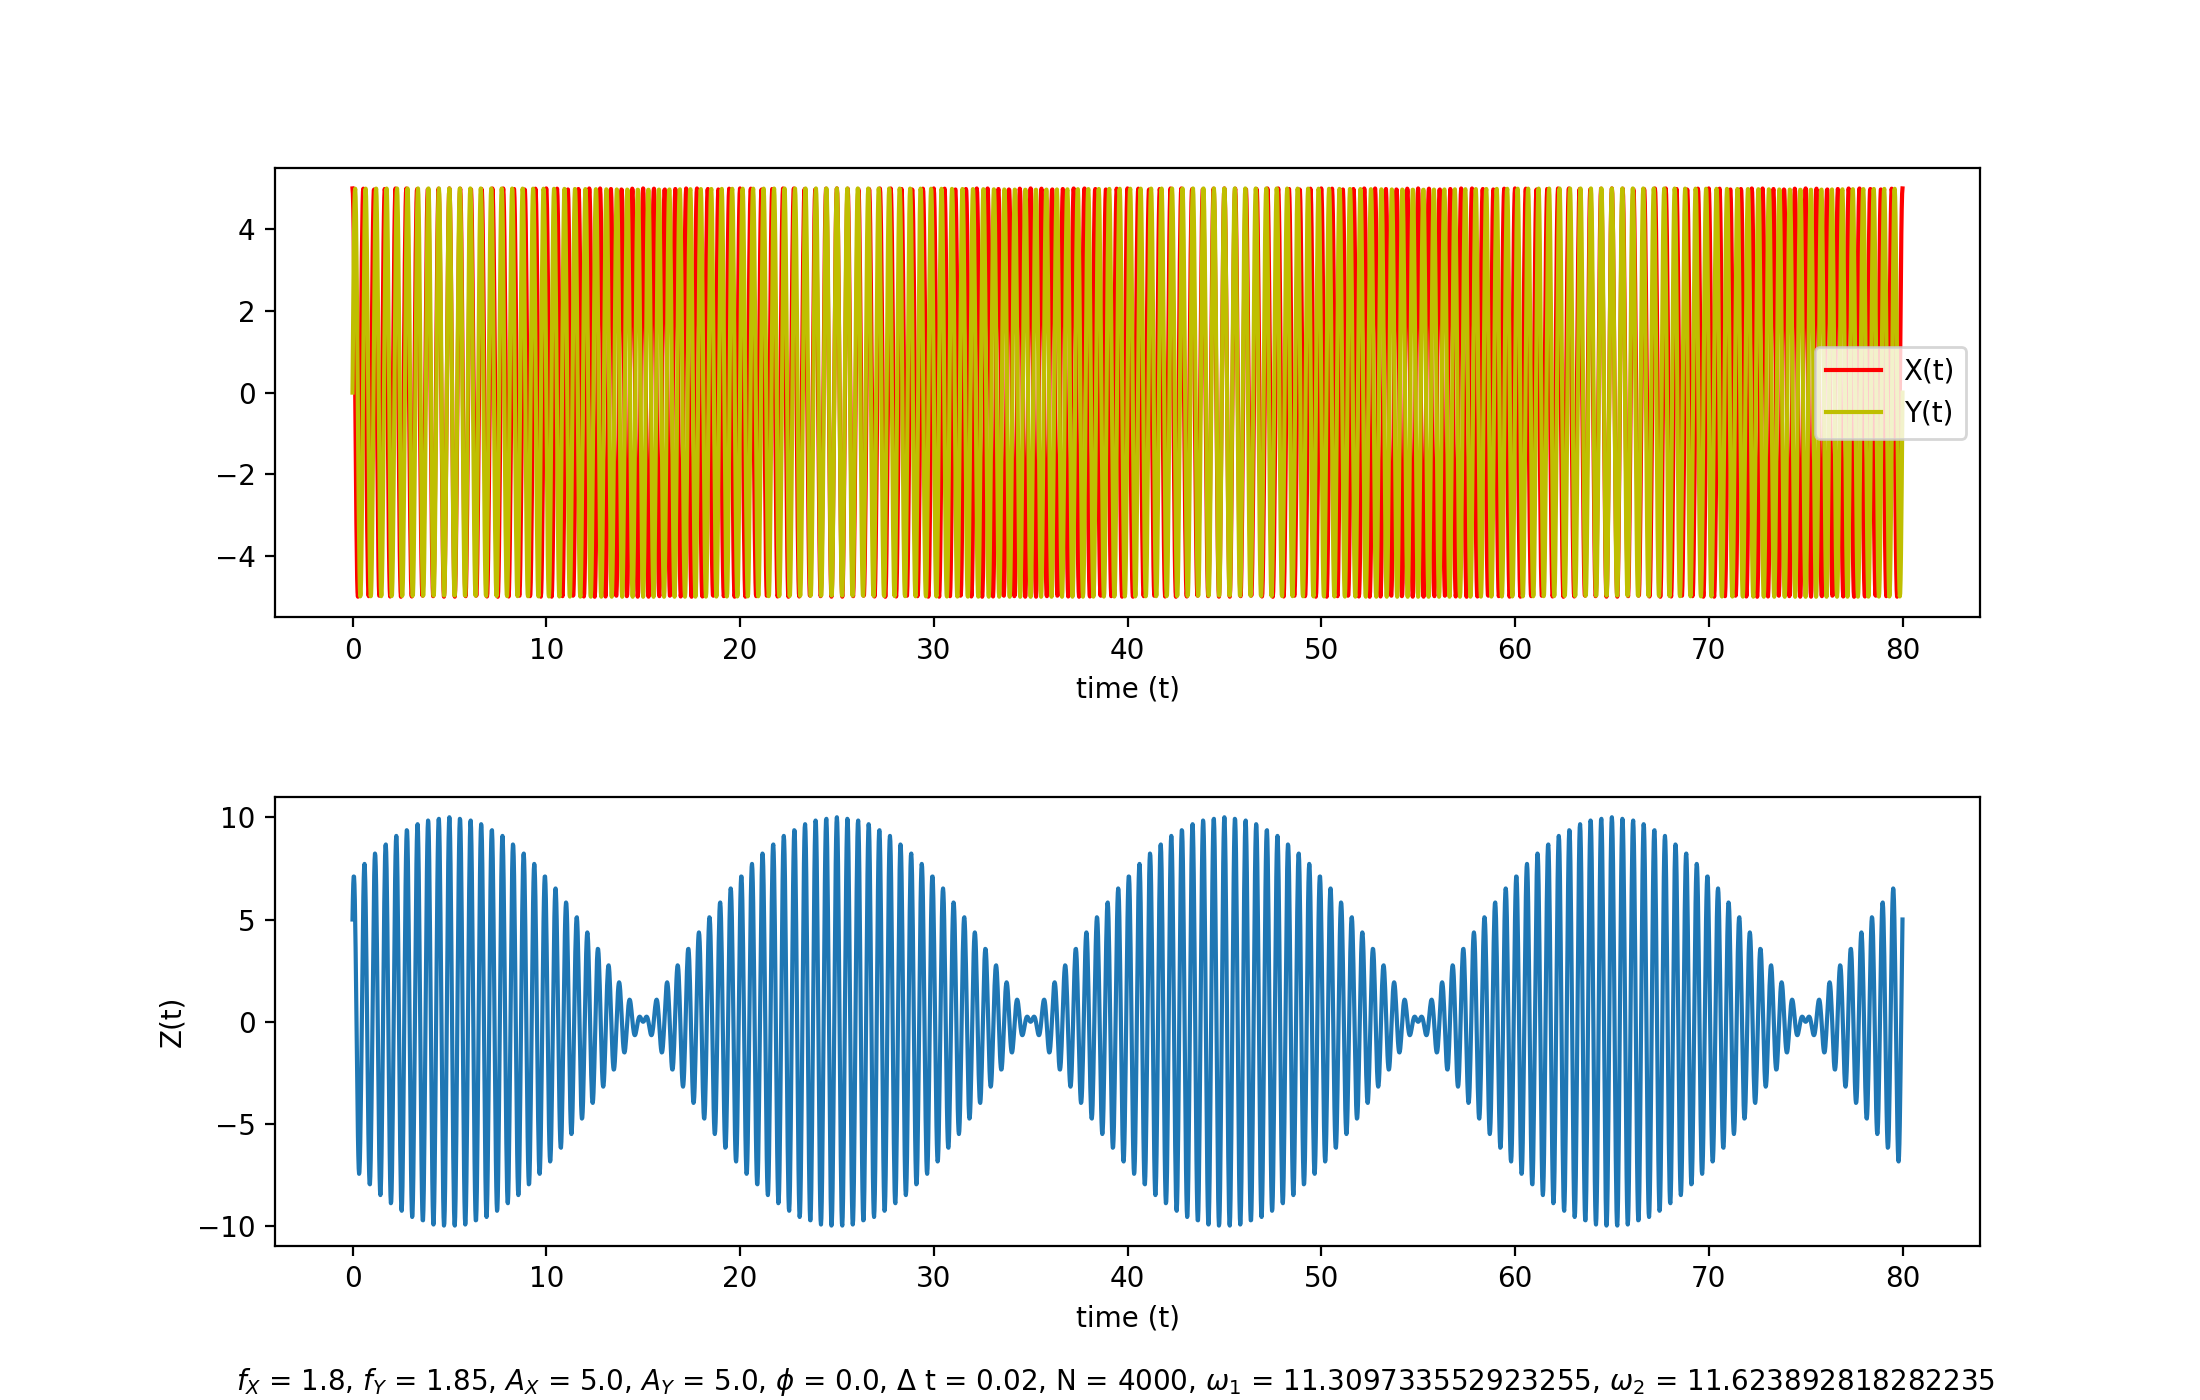
\includegraphics[width=0.48\textwidth]{41.png}}
		\subfloat[]{\label{second}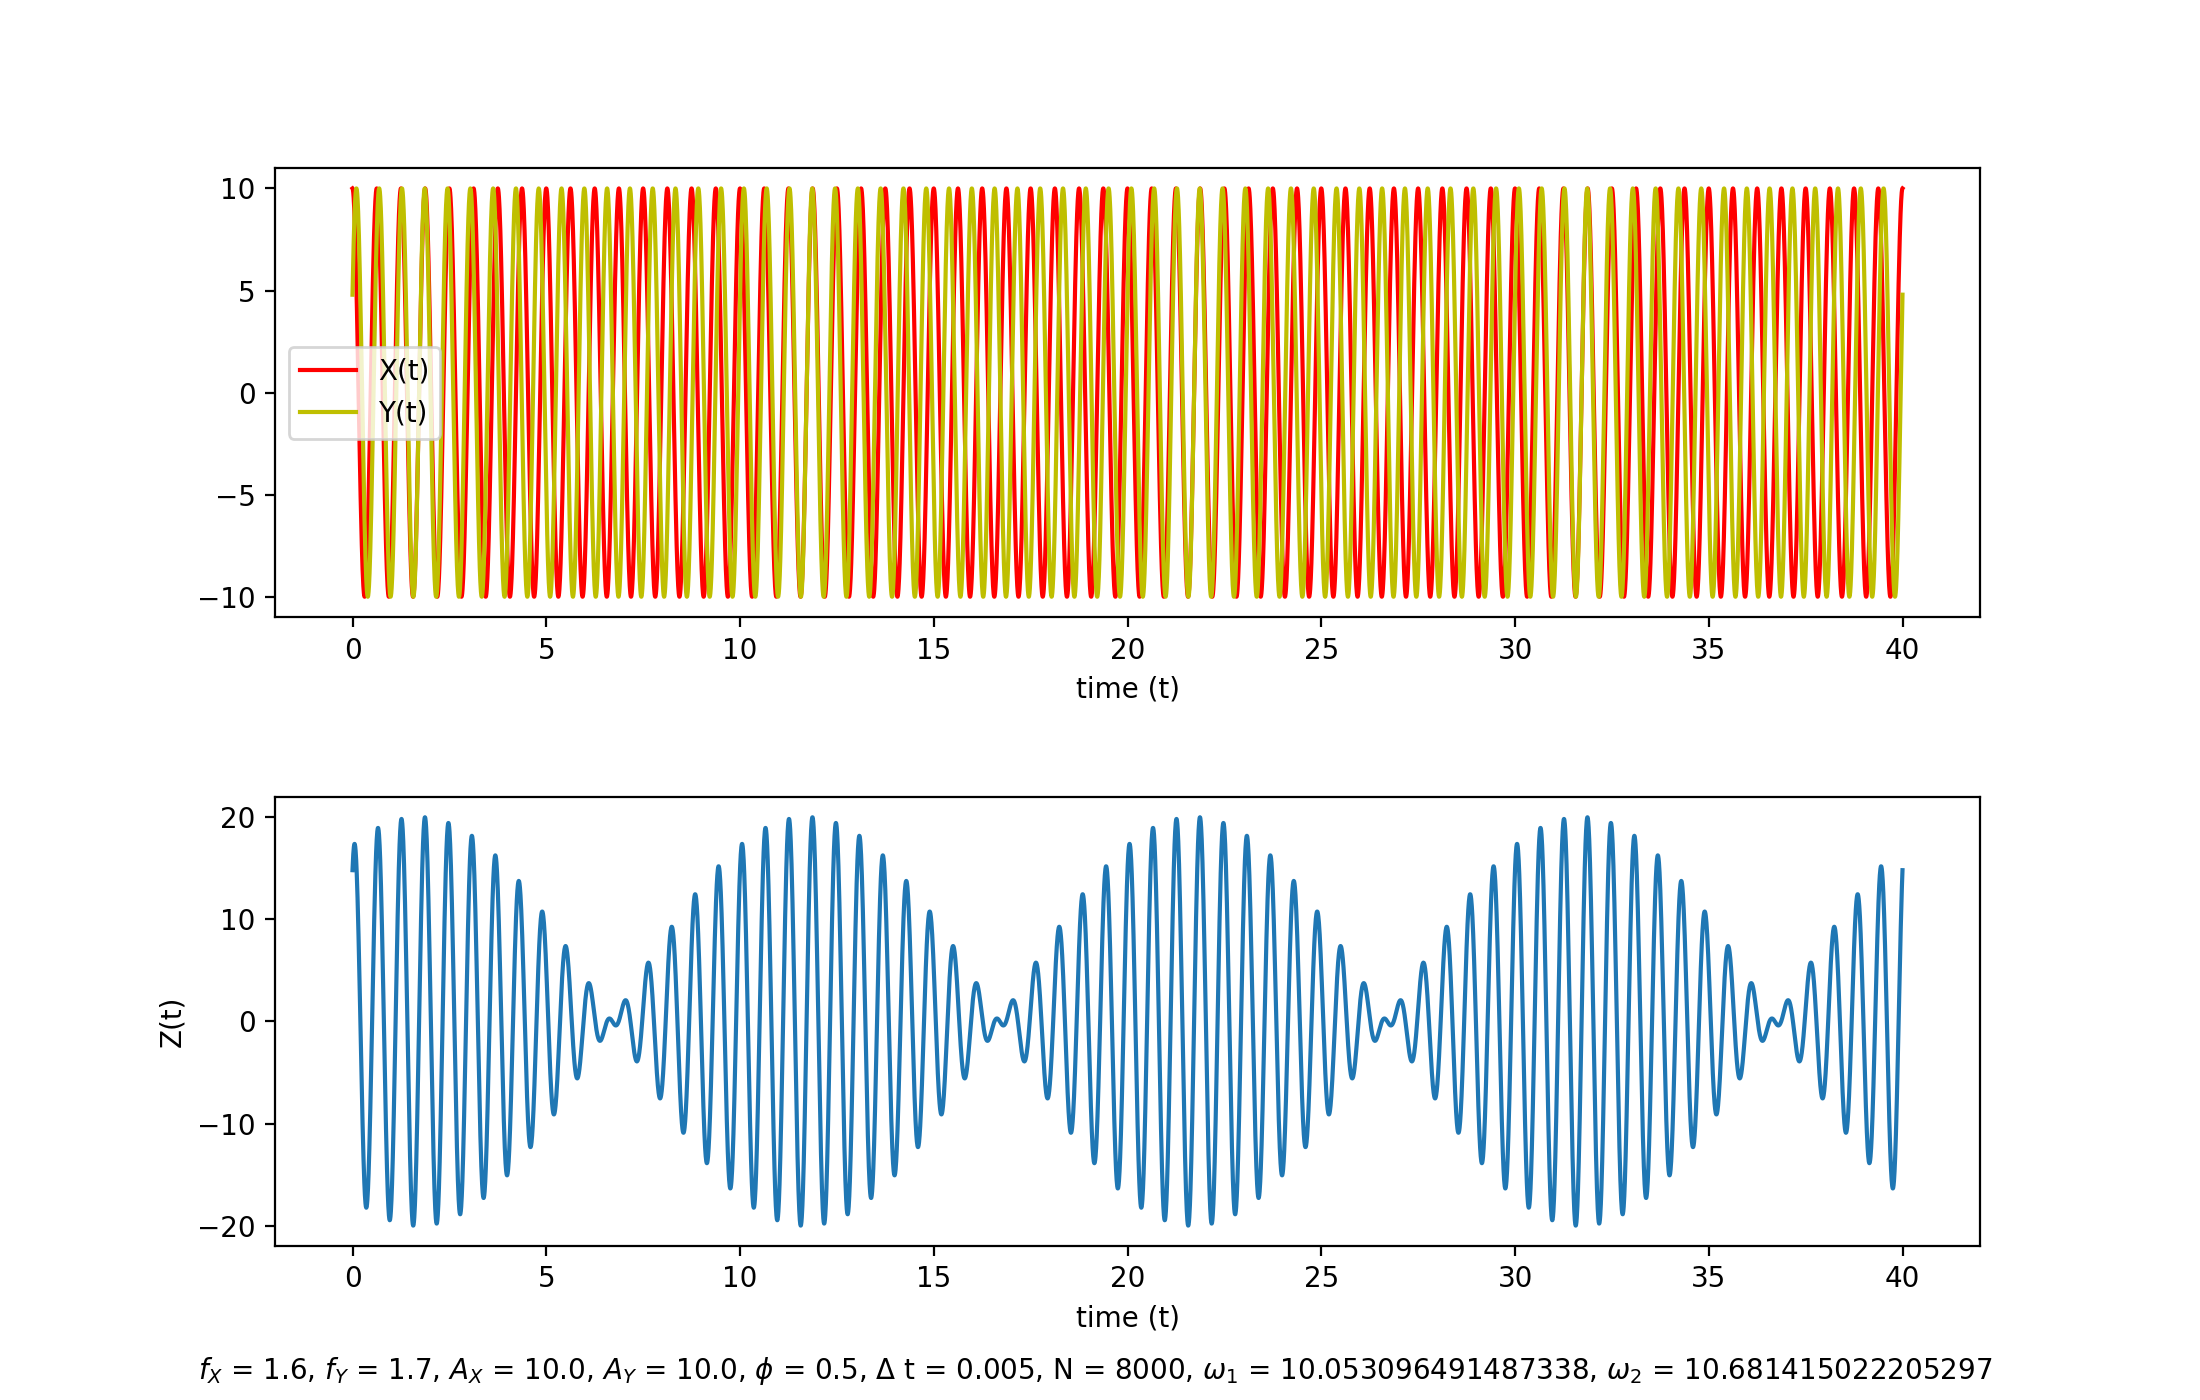
\includegraphics[width=0.48\textwidth]{42.png}}
		\caption{In both (a) and (b), $Z(t)$ displays both the carrier frequency, $\frac{\omega_1 + \omega_2}{2}$, and modulation cycles at frequency $\omega_1 - \omega_2$.}\label{fig:4}
	\end{figure}
	
	When $\phi = 0$, we can say that $X(t) + Y(t)$ is roughly $2sin(\frac{\omega_1+\omega_2}{2})cos(\frac{\omega_1\omega_2}{2})$ by the sine product-sum identity. If $2cos(\frac{\omega_1\omega_2}{2})$ is interpretted as the amplitude, the frequency includes two modulation cycles rather than one. Therefore, the frequency of the modulation cycles are at frequency $\omega_1 - \omega_2$ rather than $\frac{\omega_1 - \omega_2}{2}$. \\[4mm]
		
	\noindent\textbf{\large Problem 5}\\[2mm]
	I've had a decent amount of experience with \verb|numpy| already, but this was a nice refresher. I've had little to no experience with \verb|matplotlib| because the few times I've tried using did not turn out to be very successful. Over the past few years I've exclusively used Mathematica for plotting, although, this assignment has changed my mind about \verb|matplotlib|. I really like how customizable and straightforward plotting is in \verb|matplotlib|, so I plan to use it more often.\\
	The majority of my coding experience is in Python, but I also have experience in C/C++ and Java. I find Python much more user-friendly and universal than C and Java, so I tend to code strictly in Python. 
		
\end{document}